\section{Inicio}

\subsection{Introducción}

Año tras año la demanda de energía eléctrica mundial en general va en aumento, lo cual crea la necesidad de disponer de la energía eléctrica suficiente para satisfacer las demandas de consumo. Tanto o más importante como la producción energética, es lograr un máximo aprovechamiento de ésta mejorando el rendimiento de los equipos y de los propios receptores o instalaciones que consumen energía.

\subsection{Objetivo}

Dado que los paneles fotovoltaicos no entregan una potencia constante, ni corriente contante, ni tensión constante, hace falta un circuito que pueda manejarse bien dentro de ciertas variaciones.

El objetivo de este trabajo es, de entre todas las tecnologías y topologías de convertidores electrónicos, seleccionar la más apropiada, que pueda funcionar adaptándose a las variaciones de los paneles fotovoltaicos, y que sea la más eficiente para campos fotovoltaicos de alrededor de 5 kWp y quede dispuesta para que otro convertidor la inyecte a red o utilizar en DC. 

\subsection{Justificación}

En los últimos años se ha despertado un creciente interés por el estudio de los problemas que afectan a la red eléctrica y que degradan la calidad del suministro que reciben los usuarios de la misma. La problemática es muy variada dando lugar a un amplio campo de estudio que, entre otros muchos temas incluye los efectos de la creciente deslocalización de los sistemas de generación, debido a la gran expansión de las energías renovables, y el desarrollo de equipos de compensación activa para la mejora de la calidad del suministro y el ahorro energético.

En este informe se desarrolla el caso del convertidor semi puente boost compacto, adjunto en la \hyperref[fig:topologiareferencia]{figura 1}.

\begin{figure}
	\centering
	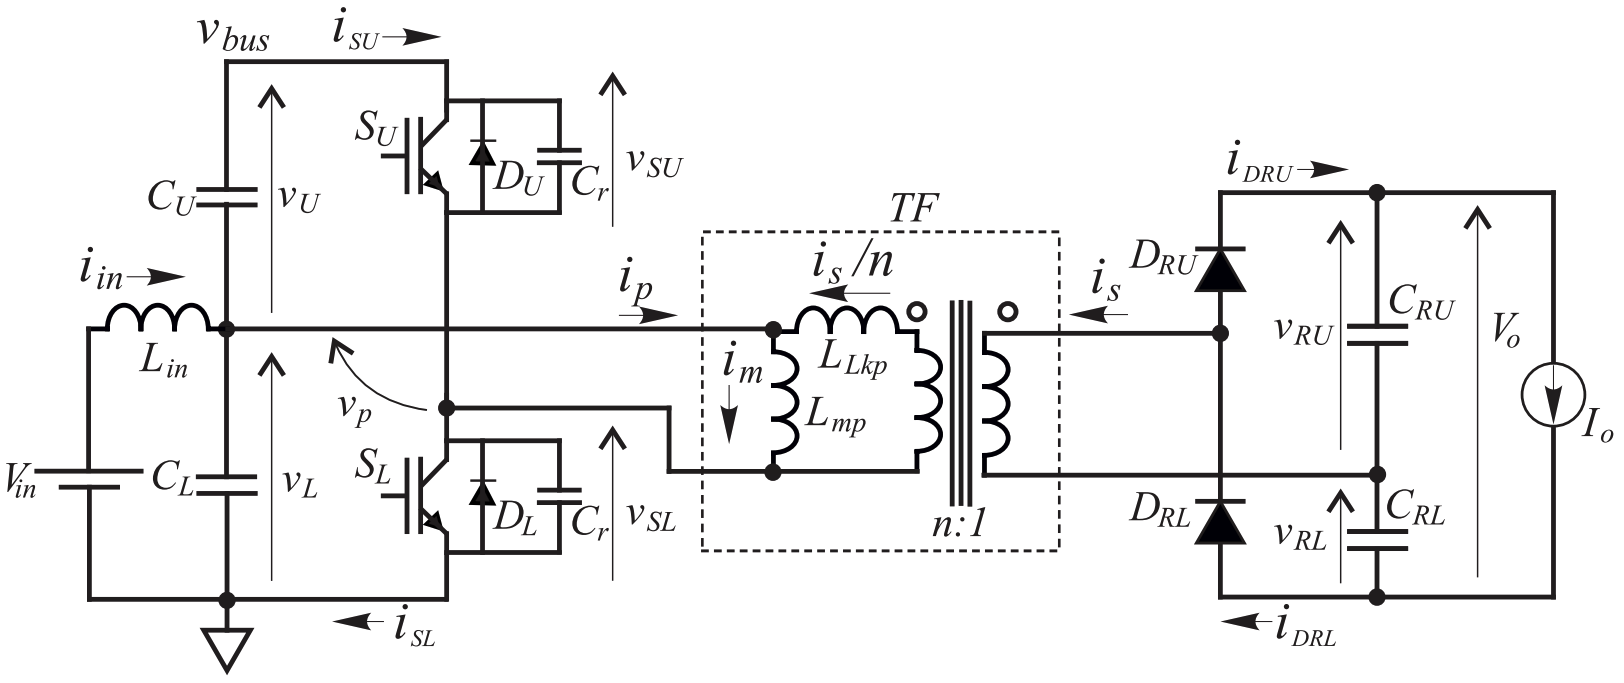
\includegraphics[width=0.9\linewidth]{img/topologiaReferencia}
	\caption[]{Convertidor semipuente boost compacto.}
	\label{fig:topologiareferencia}
\end{figure}

\subsection{Requerimientos de diseño}

\begin{itemize}
	\item Tensión de entrada: $48 \ V_{DC}$
	\item Tensión de salida: $400 \ V_{DC}$
	\item Rango de corriente: $0-40 \ A$
	\item Se pueden colocar módulos DC-DC en paralelo.
\end{itemize}

\clearpage


\section{Marco teórico}

\subsection{Descripción general}

A la entrada del convertidor se conectan los paneles solares, modelados a través de una fuente de tensión constante $V_{in}$. El inductor de entrada se usa para atenuar el ripple en la corriente de entrada $i_{in}$. Dependiendo del requerimiento de ripple en la corriente de entrada, o de la impedancia de salida de la fuente de alimentación es posible eliminar o despreciar el efecto del inductor $L_{in}$. Se usa un transformador de elevador que permita obtener la tensión de salida deseada para el requerimiento de diseño, partiendo de la alimentación a utilizar. Es posible también utilizarlo en una relación $1:1$ si simplemente es necesario un aislamiento. Es posible modelar también el transformador con su inductancia de dispersión $L_{LKp}$ y su inductancia de magnetización $L_{mp}$ referidas al primario.

Se une uno de los bornes del devanado primario del transformador con el nodo entre los capacitores de entrada $C_U$ y $C_L$, siendo que su tensión respecto de tierra es como una fuente de alimentación obtenida a partir de la carga del capacitor $C_L$ y valor $v_L$.  Se tiene una rama con transistores IGBT, formada por un dispositivo superior y otro inferior. Se tienen diodos de recuperación inversa en ambas, que pueden ser los incluidos dentro del mismo encapsulado. Se trabaja con modulación PWM a una frecuencia de conmutación $f_s=1/T_s$. Es importante dejar un pequeño tiempo muerto antes del encendido de cada uno de los IGBT, de modo de evitar un cortocircuito con la fuente. El otro extremo del transformador se conecta entre los IGBT, y tiene una tensión media $v_{SL}$ con respecto al terminal de tierra, conmutando de esa forma entre $v_{bus}$ y GND.

Se tiene así entonces para la tensión del primario $v_P$:

\begin{itemize}
	\item $v_L$ cuando el IGBT inferior está cerrado.
	\item $-v_U$ cuando el IGBT superior está cerrado.
\end{itemize}

Se tiene la salida del secundario del transformador conectada a un rectificador doblador de tensión con los diodos $D_{RL}$ y $D_{RU}$, y por los capacitores $C_{RU}$ y $C_{RL}$, estos últimos filtran la tensión de salida $V_o$, y brindando de acuerdo a la solicitud de la carga una determinada $I_o$. La energía promedio se extrae del panel solar a través del valor medio de $i_P$ del primario del transformador. Se tiene que el valor promedio $\overline{i}_{in}$ de la corriente de la fuente, igual al promedio $\overline{i}_P$.

Partiendo del ciclo de trabajo, si \( d \), tal que \( 0 < d < 1 \), representa el ciclo de trabajo del interruptor \( S_U \), el valor promedio de la tensión en el punto medio de la pierna durante \( T_s \) está dado por \(\overline{v}_{SL} = d\overline{v}_{bus}\), donde \(\overline{v}_{bus}\) es el valor promedio de \( v_{bus} \) durante \( T_s \). En régimen estacionario, los valores promedios de las caídas de tensión sobre el inductor \( L_{in} \) y sobre la inductancia de magnetización \( L_{mp} \) deben ser cero. Por consiguiente, el valor promedio de la tensión sobre el interruptor \( S_L \) es igual al valor promedio de la tensión sobre el capacitor \( C_L \) y a la tensión de la fuente de alimentación, es decir:

\[
\overline{v}_{SL} = \overline{v}_{CL} = \overline{V}_{\text{in}}
\]

En conjunto con la condición \(\overline{v}_{SL} = d\overline{v}_{bus}\), se implica que:

\[
\overline{v}_{bus} = \frac{V_{in}}{d}
\]

Los capacitores de amortiguación \( C_r \) mitigan el apagado de los interruptores \( S_U \) y \( S_L \), retrasando el incremento de sus correspondientes tensiones \( v_{SU} \) y \( v_{SL} \) durante el apagado.

\begin{figure}
	\centering
	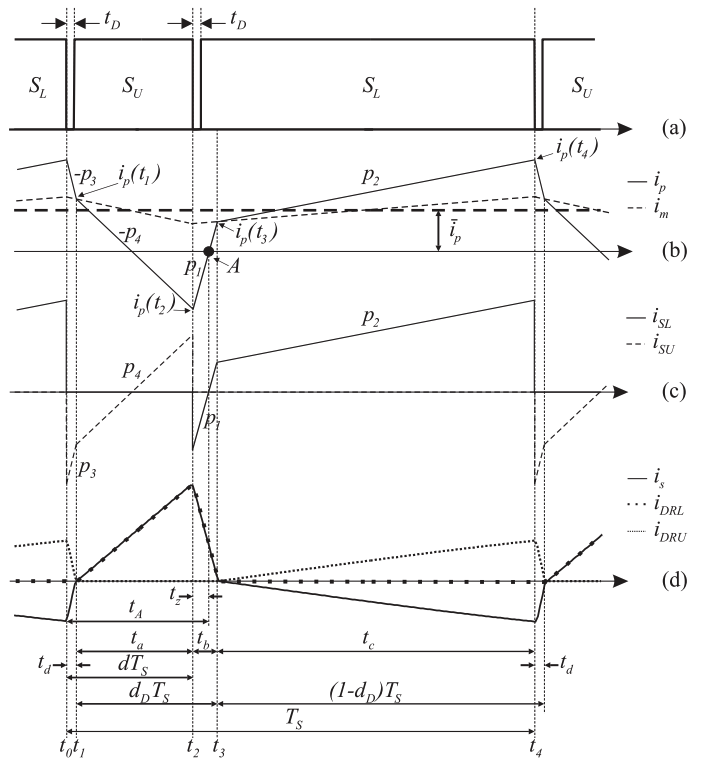
\includegraphics[width=0.7\linewidth]{img/formaOnda1}
	\caption{Formas de onda para \( d \leq 0.5 \): (a) Señales de encendido \( S_U \) y \( S_L \). (b) \( i_p \), \( \overline{i}_p \) e \( i_m \). (c) \( i_{SL} \) e \( i_{SU} \). (d) \( i_s \), \( i_{DRL} \) e \( i_{DRU} \).}
	\label{fig:formaonda1}
\end{figure}

\subsection{Operación}

Para realizar un análisis del comportamiento del convertidor en estado estacionario, se asumirá que los capacitores \( C_L \), \( C_U \), \( C_{RU} \) y \( C_{RL} \) son lo suficientemente grandes como para mantener constante la tensión sobre sus bornes durante un ciclo \( T_s \) de PWM. Por lo tanto, para este análisis, las tensiones \( v_L \) y \( v_U \) serán reemplazadas (a partir de las ecuaciones (3-1) y (3-2)) por fuentes de tensión constante de valor \( V_{in} \) y \( V_U = \frac{V_{in}(1 - d)}{d} \), respectivamente, que corresponden a sus valores medios en estado estacionario. De igual manera, las tensiones \( v_{RU} \) y \( v_{RL} \) serán reemplazadas por las tensiones constantes \( V_{RU} \) y \( V_{RL} \), que corresponden a sus valores medios teóricos en estado estacionario. Además, en este análisis no se considerarán los capacitores de snubber \( C_r \), por lo que se asumirá que la conmutación de corriente de un interruptor al otro se realiza de manera instantánea.

La\hyperref[fig:formaonda1]{figura 2} ilustra las formas de onda que permiten comprender el funcionamiento del circuito del convertidor. Como se puede observar, estas figuras corresponden al convertidor operando con un ciclo de trabajo del interruptor \( S_U \), \( d < 0.5 \). La \hyperref[fig:formaonda1]{figura 2}(a) ilustra las señales de encendido de los interruptores \( S_U \) y \( S_L \). Nótese la introducción de tiempos muertos de duración \( t_D \) entre el apagado y el encendido de ambos interruptores. La \hyperref[fig:formaonda1]{figura 2}(b) muestra la corriente \( i_p \) por el primario del transformador, su valor medio \( \overline{i}_p \), y la corriente de magnetización \( i_m \). En la \hyperref[fig:formaonda1]{figura 2}(c) se presentan las formas de onda de las corrientes \( i_{SL} \) e \( i_{SU} \) a través de los interruptores \( S_L \) y \( S_U \), respectivamente; y en la \hyperref[fig:formaonda1]{figura 2}(d) las corrientes \( i_{DRL} \) e \( i_{DRU} \) a través de los diodos del rectificador, y la corriente \( i_s \) por el secundario del transformador.

\subsection{Modos de operación}

Se analiza la figura de las formas de onda de forma detallada. Para eso, se parte del hecho de que durante un período de conmutación, o sea, $T_s$, el convertidor tiene cuatro modos de operación que corresponden a los ilustrados en la \hyperref[fig:modosoperacion]{figura 4}.

\begin{enumerate}
	\item Modo 1 (Periodo \( t_d = t_1 - t_0 \))
	\item Modo 2 (Periodo \( t_a = t_2 - t_1 \))
	\item Modo 3 (Periodo \( t_b = t_3 - t_2 \))
	\item Modo 4 (Periodo \( t_c = t_4 - t_3 \))
\end{enumerate}

\begin{figure}
	\centering
	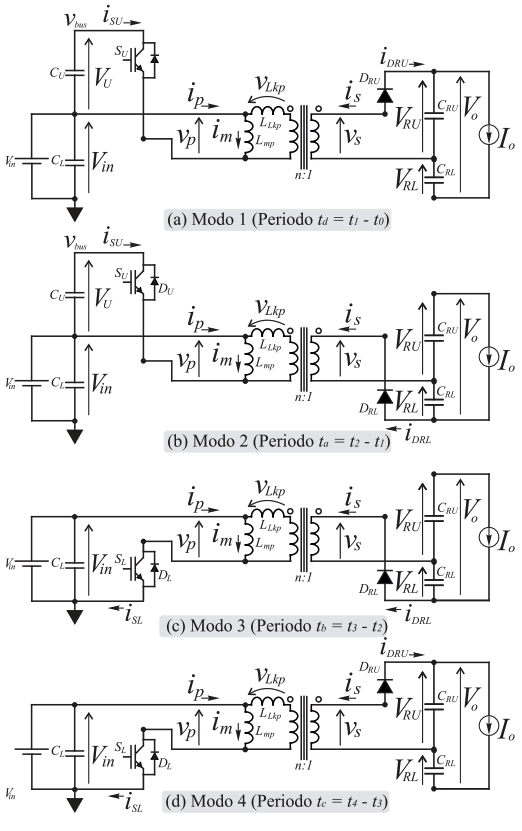
\includegraphics[width=0.7\linewidth]{img/modosOperacion}
	\caption{Modos de operación del convertidor.}
	\label{fig:modosoperacion}
\end{figure}


\subsubsection{Modo 1}

En el instante \( t_0 \), cuando se apaga el interruptor \( S_L \), la corriente \( i_p \) alcanza su valor máximo positivo \( i_p(t_0) \) y pasa instantáneamente a circular por el diodo  \( D_U \) del interruptor \( S_U \). El circuito correspondiente a este intervalo se muestra en la Fig. 3-4(a). En este modo de operación, la tensión aplicada al primario del transformador es \( v_p = -V_U \). La corriente del secundario circula por el diodo \( D_{RU} \), aplicando una tensión \( v_s = V_{RU} \) al secundario del transformador, y una tensión \( v_{LKp} = -(V_U + nV_{RU}) \) sobre la inductancia de dispersión. Así, durante este intervalo, la corriente \( i_m \) decrece con pendiente \( -V_U / L_{mp} \) y la corriente por la inductancia de dispersión decrece con pendiente \( -(V_U + nV_{RU}) / L_{LKp} \). La corriente \( i_p \) por el primario del transformador (suma de la corriente por la inductancia de magnetización y la corriente por la inductancia de dispersión) decrece con pendiente:

\[
-p_3 = -\left( \frac{V_U}{L_p} + n \frac{V_{RU}}{L_{LKp}} \right)
\]

donde \( L_p = L_{LKp} \parallel L_{mp} \). Luego del intervalo \( t_D \) (tiempo muerto), contado a partir de \( t_0 \), se activa el gate del IGBT \( S_U \). El encendido de \( S_U \) se realiza a tensión y corriente cero, pues \( i_p \), que es positiva, circula en ese instante por el diodo en antiparalelo con \( S_U \), evitando pérdidas de conmutación. Este modo finaliza en el instante \( t_1 \), cuando la corriente \( i_p \) iguala a la corriente \( i_m \), momento en el que \( D_{RU} \) se apaga naturalmente cuando su corriente se hace cero.

\subsubsection{Modo 2}

Al inicio de este modo de operación, la corriente que circula por el primario del transformador es igual a la corriente por la inductancia de magnetización, con un valor de \( i_p(t_1) \). Después del instante \( t_1 \), la corriente \( i_p \) se vuelve menor que la corriente de magnetización \( i_m \), haciendo que la corriente del secundario circule por el diodo \( D_{RL} \). . La corriente \( i_{DRL} \) crece desde cero con una pendiente limitada, evitando pérdidas durante el encendido del diodo \( D_{RL} \). La tensión aplicada sobre la inductancia de magnetización sigue siendo \( v_p = -V_U \), mientras que la tensión en el secundario del transformador es \( v_s = -V_{RL} \). Por lo tanto, la corriente \( i_m \) decrece con pendiente \( -\frac{V_U}{L_{mp}} \) y la corriente por la inductancia de dispersión decrece con pendiente \( -\frac{V_U - nV_{RL}}{L_{LKp}} \). La corriente \( i_p \) decrece con pendiente:

\[
-p_4 = -\left( \frac{V_U}{L_p} + n \frac{V_{RL}}{L_{LKp}} \right)
\]

donde \( L_p = L_{LKp} \parallel L_{mp} \). El Modo 2 finaliza en \( t_2 = dT \), cuando se apaga el IGBT \( S_U \).

\subsubsection{Modo 3}

Cuando se apaga el IGBT \( S_U \), la corriente \( i_p \) alcanza su máximo negativo \( i_p(t_2) \) y pasa instantáneamente a circular por \( D_L \) del IGBT \( S_L \). El diodo \( D_{RL} \) del rectificador permanece en conducción, y su corriente comienza a decrecer. La tensión sobre la inductancia de magnetización del transformador pasa a ser \( v_p = V_{in} \), mientras que la tensión en el secundario sigue siendo \( v_s = -V_{RL} \). La corriente \( i_m \) crece con pendiente \( \frac{V_{in}}{L_{mp}} \), y la corriente por la inductancia de dispersión crece con pendiente \( \frac{V_{in} + nV_{RL}}{L_{LKp}} \). La corriente por el primario crece con la pendiente:

\[
p_1 = \left( \frac{V_{in}}{L_p} + n \frac{V_{RL}}{L_{LKp}} \right)
\]

donde \( L_p = L_{LKp} \parallel L_{mp} \). Para asegurar el encendido a tensión y corriente cero de \( S_L \), la activación de este IGBT debe hacerse antes de que la corriente \( i_p \) cambie de signo. Esta es una condición de diseño para el correcto funcionamiento del convertidor, asegurando que en el instante de activación la corriente esté circulando por el diodo de recuperación inversa \( D_L \). Este modo finaliza en el instante \( t_3 \) cuando la corriente \( i_p \) iguala a la corriente \( i_m \), momento en el que el diodo \( D_{RL} \) del rectificador se apaga naturalmente al alcanzar su corriente cero.

\subsubsection{Modo 4}

Durante este intervalo, la corriente \( i_p \) que entra al primario del transformador supera a la corriente de magnetización \( i_m \), lo que lleva al encendido del diodo \( D_{RU} \). Este modo de operación coincide con el circuito ilustrado en la Figura 3-4(d). La tensión en el primario del transformador permanece como \( v_p = V_{in} \), mientras que la tensión en el secundario se convierte en \( v_s = V_{RU} \). La corriente \( i_m \) aumenta con una pendiente de \( \frac{V_{in}}{L_{mp}} \), y la corriente a través de la inductancia de dispersión aumenta con una pendiente de \( \frac{V_{in} - nV_{RU}}{L_{LKp}} \). La corriente \( i_p \) también aumenta con una pendiente dada por:

\[
p_2 = \left( \frac{V_{in}}{L_p} - n \frac{V_{RU}}{L_{LKp}} \right)
\]

donde \( L_p = L_{LKp} \parallel L_{mp} \) (3-6). Este modo de operación concluye en \( t_4 = T_s \), momento en que se apaga el IGBT \( S_L \) y se reinicia al Modo 1.

\subsection{Estado estacionario}

Para caracterizar a un convertidor como el trabajado en este informe, se desea conocer su ganancia en tensión $V_o/V_{in}$. Se sabe que este circuito no tiene un comportamiento lineal, por lo que no se puede hallar una ecuación cerrada que exprese la ganancia. Para ello, se toma como referencia del material bibliográfico, un estudio realizado, que obtiene de manera analítica un conjunto de cuatro ecuaciones no lineales con cuatro incógnitas, que definen el comportamiento del convertidor en estado estacionario y permiten encontrar su ganancia de tensión para cualquier punto de operación. Para no depender de la relación de transformación, se trata con las tensiones intervinientes referidas al primario del transformador. 

Se tiene la siguiente \hyperref[fig:corrienteestacionario]{característica de la forma de onda de corriente para estado estacionario}.

\begin{figure}
	\centering
	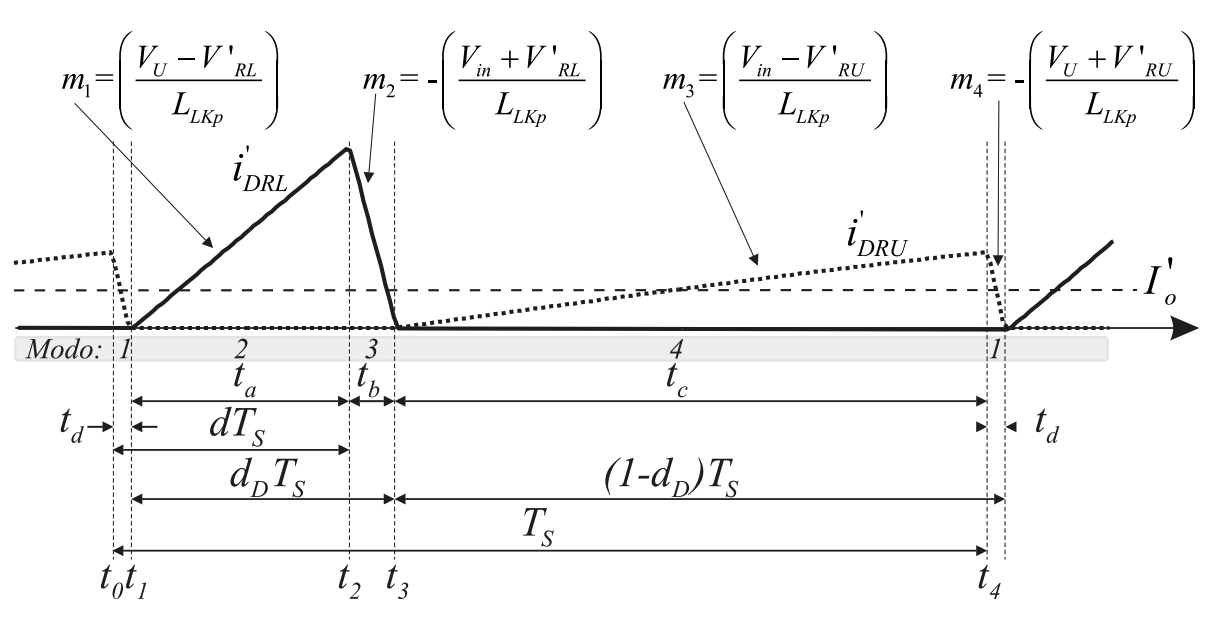
\includegraphics[width=0.7\linewidth]{img/corrienteEstacionario}
	\caption{Corrientes del circuito en estado estacionario.}
	\label{fig:corrienteestacionario}
\end{figure}

En donde las pendientes están dadas por:

$$
\begin{cases}
	m_1 = \frac{V_U - V_0}{R_L L_{LKp}} \\
	m_2 = -\frac{V_{in} + V_0}{R_L L_{LKp}} \\
	m_3 = \frac{V_{in} - V_0}{R_U L_{LKp}} \\
	m_4 = -\frac{V_U + V_0}{R_U L_{LKp}}
\end{cases}
$$

Finalmente, las cuatro incógnitas son:

\begin{itemize}
	\item $V_{RU}'$
	\item $V_{bus}$
	\item $t_b$
	\item $t_d$
\end{itemize}

Siendo posible resolver de forma numérica ecuaciones para obtener valores para cada punto específico de operación dado por:

\begin{itemize}
	\item $V_{in}$
	\item $I_o'$
	\item $V_o'$
\end{itemize}

Y a partir de esto obtener la relación $V_o'/V_{bus}$ deseada. Entonces, el sistema de cuatro ecuaciones que modelan el comportamiento del convertidor es:

$$
\begin{cases}
	[V_{bus(pu)}-V_{in(pu)}-(V'_{o(pu)}-V'_{RU(pu)})]\frac{V'_{RU(pu)}}{V'_{o(pu)}}T_{s(pu)}=V_{bus(pu)}t_{b(pu)} \\
	(V_{in(pu)}-V'_{RU(pu)})\left(\frac{V'_{o(pu)}-V'_{RU(pu)}}{V'_{o(pu)}}\right)T_{s(pu)}=V_{bus(pu)}t_{b(pu)} \\
	I'_{o(pu)} = \frac{V'_{RU(pu)}}{2V'_{o(pu)}} \left(\frac{V_{in(pu)}+V'_{o(pu)}-V'_{RU(pu)}}{L_{LKp(pu)}}\right) 2\pi t_{b(pu)} \\
	I'_{o(pu)} = \frac{V'_{o(pu)}-V'_{RU(pu)}}{2V'_{o(pu)}} \left(\frac{V_{bus(pu)}-V_{in(pu)}+V_{RU(pu)}}{L_{LKp(pu)}}\right)2\pi t_{d(pu)}\
\end{cases}
$$

Se logran las siguientes curvas de regulación para las ecuaciones anteriores.

\begin{figure}
	\centering
	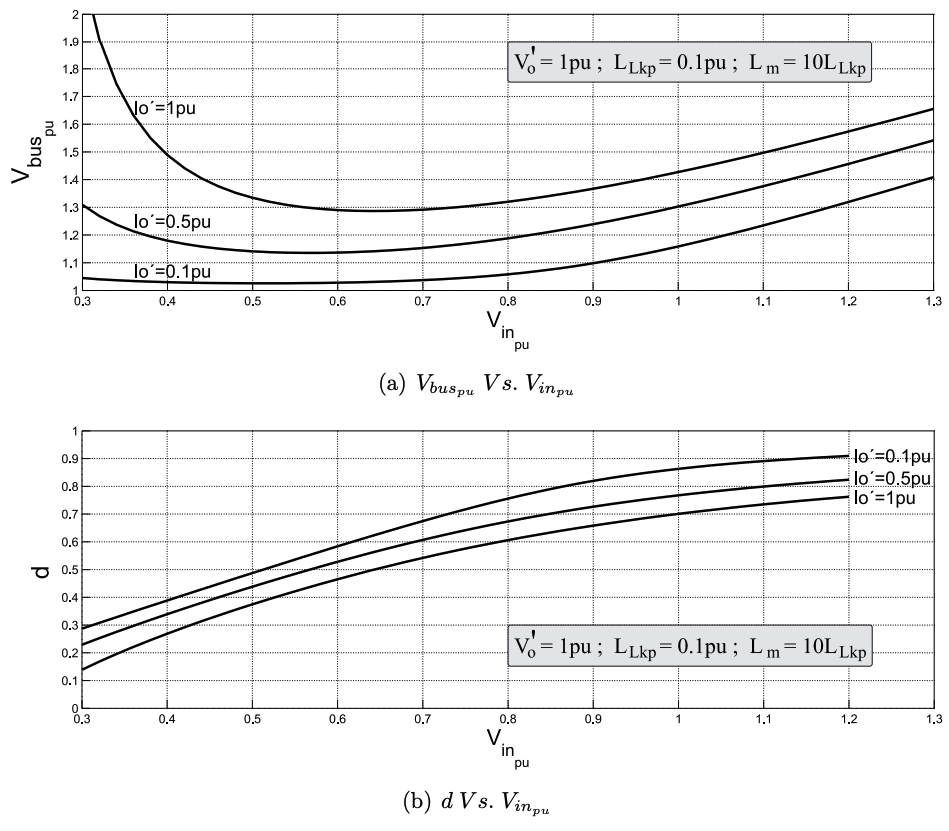
\includegraphics[width=0.9\linewidth]{img/eqV}
	\caption{(a) $d \ vs. \ V_{in(pu)}$ y (b) $V_{bus(pu)} \ vs. \ V_{in(pu)}$; para $V'_{o(pu)}=1$ parametrizada en $I'_{o(pu)}$.}
	\label{fig:eqv}
\end{figure}

\begin{figure}
	\centering
	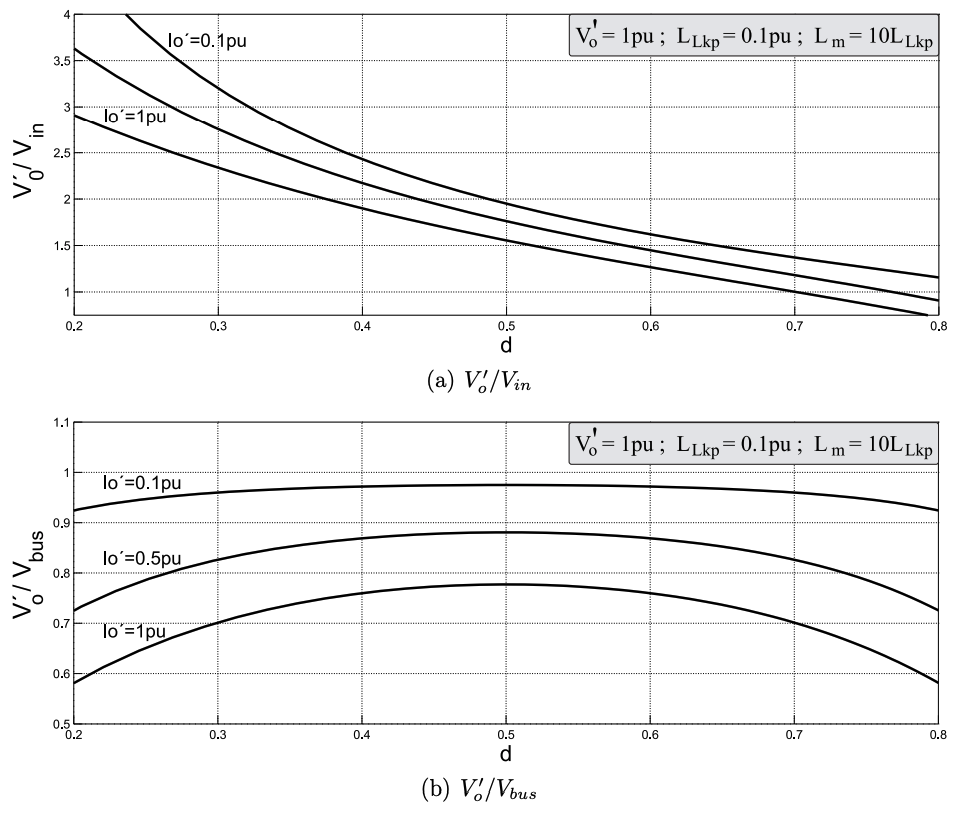
\includegraphics[width=0.9\linewidth]{img/eqI}
	\caption{Ganancias del convertidor en función del ciclo de trabajo $d$ y de la corriente de salida $I'_{o(pu)}$.}
	\label{fig:eqi}
\end{figure}


\subsection{Conmutación suave}

También llamada ZVS (Zero Voltage Switching), se puede lograr bajo cierta condiciones y con un determinado rango de tensión de entrada y corriente de salida. El rango de conmutación suave está definido por la relación entre la inductancia de magnetización y la inductancia de dispersion del transformador $L_{mp}/L_{LKp}$, por el valor de los capacitores de snubber $C_r$ y el tiempo muerto $t_D$ entre el apagado de un IGBT y el encendido del otro.

\subsubsection{Encendido a tensión cero de $S_U$}

Esto es fácil de lograr, cuando se apaga $S_L$, $i_P$ pasa a circular por el diodo $D_U$, haciendo que la tensión se vaya a cero. En este momento $i_P$ está en su máximo valor positivo, por lo que se tiene un tiempo considerable para encender $S_U$ antes de que la corriente cambie de signo y despolarice el diodo $D_U$.

\subsubsection{Encendido a tensión cero de $S_L$}

Este encendido es más crítico que el anterior. En el instante $t_2$, cuando se apaga $S_U$, la corriente $i_P$ alcanza su mínimo y pasa a circular por el diodo $D_L$. La magnitud mínima $i_P(t_2)$ puede ser pequeña y a partir de ese momento la corriente por el primario del transforamdor comienza a crecer con una pendiente elevada, $p_1$. De esta forma, el tiempo muerto $t_D$ máximo a usar es reducido.

\begin{figure}
	\centering
	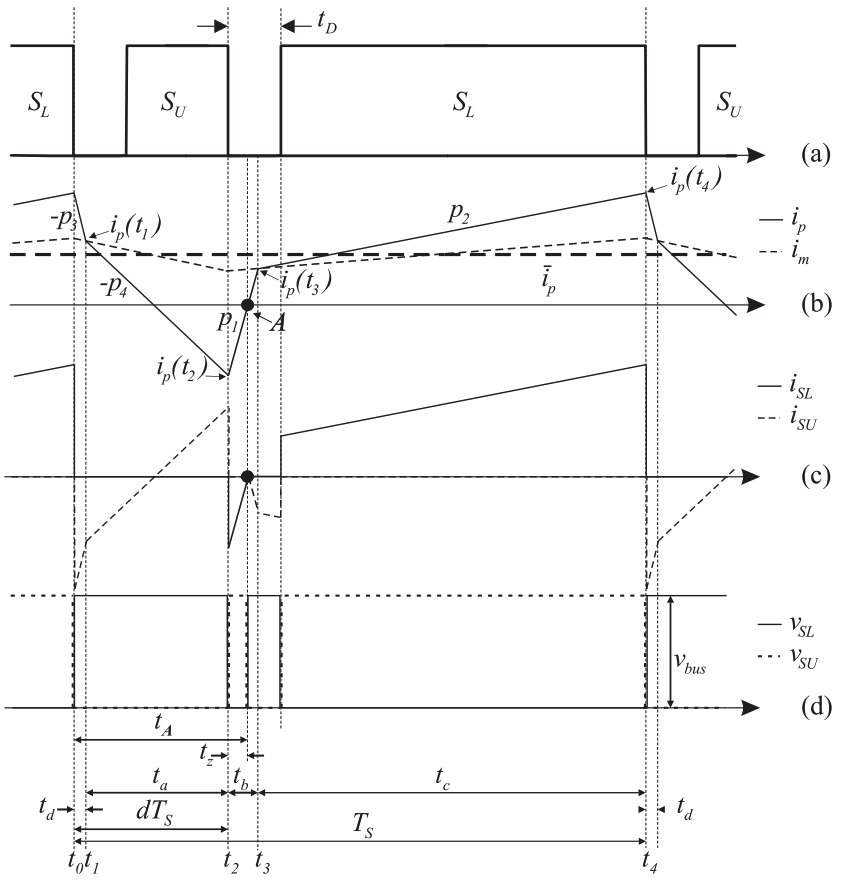
\includegraphics[width=0.7\linewidth]{img/suave1}
	\caption{Curvas para \( t_D > t_z \): (a) Señales de encendido $S_U$ y $S_L$. (b) \( i_p \), \( \bar{i}_p \) e \( i_m \). (c) \( i_{SL} \) e \( i_{SU} \). (d) \( v_{SL} \) y \( v_{SU} \).}
	\label{fig:suave1}
\end{figure}

\subsubsection{Tiempo muerto $t_D$}

Luego del apagado de la llave $S_U$, para asegurar que la llave $S_L$ encienda a tensión cero, su activación debe realizarse antes de que $i_P$ cambie de negativa a positiva. Si se define $t_A$ como el tiempo contado desde $t_0$, hasta el instante en que la corriente cruza por cero en el punto A, y se define $t_z=(t_A-t_2)$ como el tiempo que tarda la corriente $i_P$ en cruzar por cero luego del momento $t_2$ en que se apagó $S_U$, para que la llave $S_L$ encienda a tensión cero, debe ser $t_D<t_z$.

\begin{figure}
	\centering
	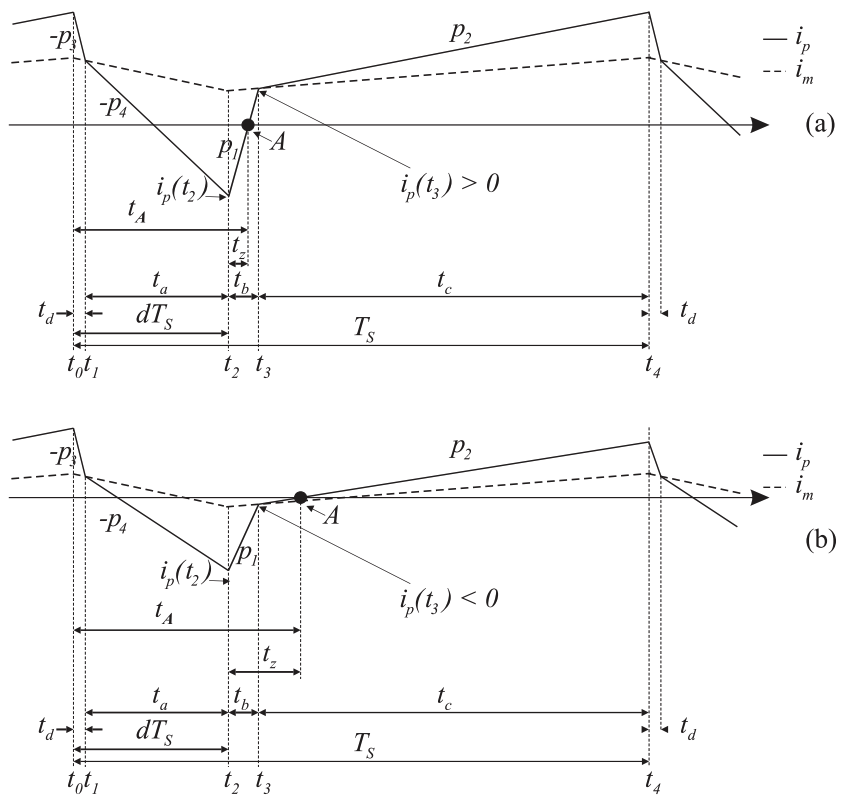
\includegraphics[width=0.8\linewidth]{img/tD}
	\caption{Forma de onda de las corrientes $i_P$ e $i_m$ para: (a) $i_m(t_3)>0$ y (b) $i_m(t_3)<0$.}
	\label{fig:td}
\end{figure}

Resulta necesario limitar el valor mínimo de la relación $L_{mp}/L_{LKp}$, además, al aumentar esta relación disminuye $t_{z(min)}$. Esto no es conveniente porque limita el tiempo muerto $t_D$, que es el tiempo que tienen las llaves en el apagado para llevar a cero las corrientes y realizar la carga o descarga de los capacitores de snubber. Por eso se define como relación de compromiso $L_{mp}/L_{LKp}=10$. Siendo que, para que el convertidor opere en conmutación suave en todo el rango $0.42<V_{in(pu)} < 0.9$, debe utilizarse un tiempo muerto $t_D\leq 0.48 \ \mu s$.

\subsubsection{Efecto de los capacitores de snubber $C_r$}

Los capacitores de snubber tienen la función de retardar el aumento de la tensión sobre las llaves $S_L$ y $S_U$ durante su apagado. Esto es esencial porque las llaves no pueden apagarse instantáneamente, sino que requieren un tiempo finito, conocido como tiempo de caída. Durante este período, es crucial retrasar el aumento de la tensión para minimizar las pérdidas. Aunque es deseable que los capacitores de snubber sean grandes para maximizar este retardo, se debe tener cuidado. Un exceso de tamaño podría retrasar también la caída de tensión en la llave próxima a encenderse, lo que resultaría en pérdidas adicionales durante su encendido.

\begin{figure}
	\centering
	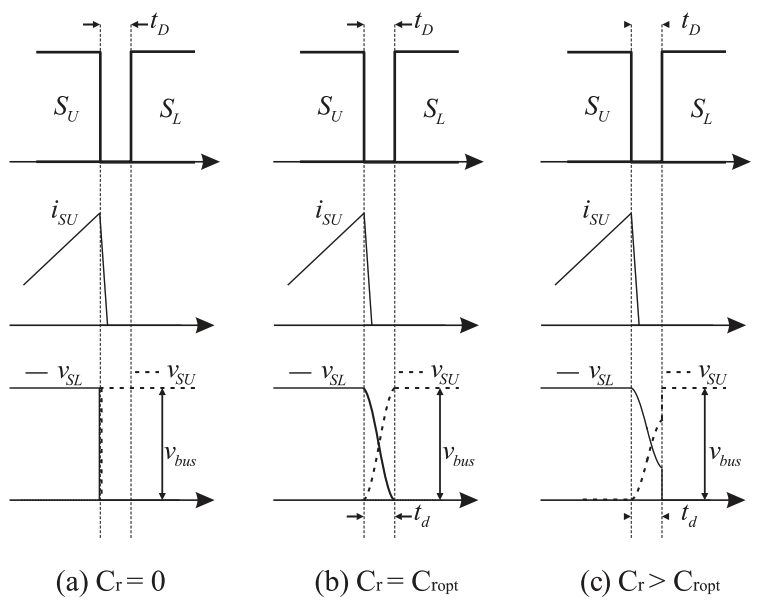
\includegraphics[width=0.6\linewidth]{img/capSnubber}
	\caption{Señales de encendido de $S_L$ y $S_U$, corriente $i_{SU}$ y tensiones $v_{SU}$ para distintos casos de valores de capacitancia de snubber.}
	\label{fig:capsnubber}
\end{figure}

Para cada punto de operación del convertidor debe existir un valor óptimo de los capacitores de snubber $C_{ropt}$, que haga que la tensión sobre la llave próxima a encenderse llegue a cero justo en el instante de encendido.

\subsubsection{Diseño de los capacitores de snubber $C_r$}

\begin{figure}
	\centering
	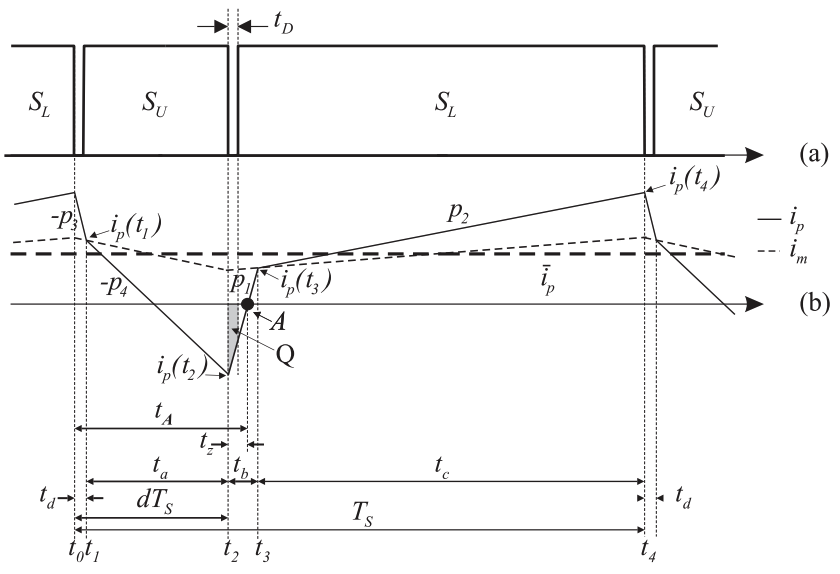
\includegraphics[width=0.6\linewidth]{img/energiaQ}
	\caption{Energía $Q$ utilizada para el dimensionamiento de los capcaitores de snubber.}
	\label{fig:energiaq}
\end{figure}

Para calcular el valor máximo que pueden tener los capacitores de snubber $C_r$, a fin de que la tensión haya llegado a cero antes de que se encuenda la llave $S_L$ en todo el rango de operación del convertidor, se calcula el área de la corriente $i_P$ durante el intervalo sombreado en la \hyperref[fig:energiaq]{figura 10}. Se define de esa manera $C_{r0}=Q/2V_{bus}$, $C_{r(pu)}=2\pi R_B C_{r0}/T_B$, aproximando de esa forma un valor $C_{r(pu)} \approx 0.02$ que asegura la conmutación suave para el rango de tensión $0.42 < V_{in(pu)} < 0.9$.


\clearpage


\section{Diseño del convertidor}

\subsection{Puntos de partida}

De las especificaciones de diseño, dadas en la consigna del desarrollo a realizar, se tiene en cuenta lo siguiente:

\begin{itemize}
	\item Se pueden conectar paneles solares en paralelo de forma de tener una mayor corriente de entrada.
	\item El uso de paneles solares en paralelo asegura continuidad del servicio ante fallas individuales de los mismos.
	\item Para lograr la salida deseada, es posible implementar convertidores en paralelo.
\end{itemize}


Las especificaciones de potencia de paneles solares, o campos fotovoltaicos viene dada en la unidad kWp, que refiere a la potencia de salida para las condiciones estándar de prueba (\textbf{STC}: \textit{Standard Test Conditions}), que son:

\begin{itemize}
	\item Irradiancia de $1000 \ W/m^2$.
	\item Temperatura de cédula de 25 grados centígrados.
	\item Masa de aire de 1.5.
\end{itemize}

Se toman entonces, como referencia, paneles solares de $550 \ W$, en este caso de la marca Panasonic, más precisamente de la línea Anchor, el modelo es AE14HXXXVHC10B, del cual se tienen las siguientes características:

\begin{table}[h]
	\centering
	\begin{tabular}{|c|c|c|c|c|c|}
		\hline
		\textbf{STC} & \textbf{550W} & \textbf{545W} & \textbf{540W} & \textbf{535W} & \textbf{530W} \\ \hline
		\textbf{Wattage, Wp} & 550W & 545W & 540W & 535W & 530W \\ \hline
		\textbf{Voltage at Max Power, Vmax} & 42.05V & 41.87V & 41.75V & 41.57V & 41.39V \\ \hline
		\textbf{Open Circuit Voltage, Voc} & 49.88V & 49.69V & 49.54V & 49.39V & 49.24V \\ \hline
		\textbf{Current at Max Power, Imax} & 13.08A & 13.02A & 12.94A & 12.87A & 12.81A \\ \hline
		\textbf{Short Circuit Current, Isc} & 14.01A & 13.96A & 13.89A & 13.83A & 13.76A \\ \hline
		\textbf{Module Efficiency} & 21.3\% & 21.1\% & 20.9\% & 20.7\% & 20.5\% \\ \hline
		\textbf{Operating Temperature (°C)} & \multicolumn{5}{c|}{-40°C ~ +85°C} \\ \hline
		\textbf{Maximum System Voltage} & \multicolumn{5}{c|}{1500 V DC (IEC)} \\ \hline
		\textbf{Maximum Series Fuse Rating} & \multicolumn{5}{c|}{25 A} \\ \hline
		\textbf{Power Tolerance} & \multicolumn{5}{c|}{0 to +5 Wp} \\ \hline
	\end{tabular}
	\caption{Especificaciones técnicas del módulo AE14HxxxVHC10B}
	\label{tab:module_specs}
\end{table}

Puede verse cómo para el módulo de $550 \ W$, se tiene una salida de tensión de alimentación máxima de $42.05 \ V$, y a circuito abierto de $49.88 \ V$. Se tomará como referencia, con el fin de cumplir los objetivos de diseño de la consigna como si el dato de $V_{max}$ fuera $48 \ V$, y se ajusta la corriente máxima a la potencia:

$$
I_{max} = \frac{550W}{48V}= 11.45A
$$

Ahora, hay ciertos aspectos a tener en cuenta, a priori, usando el dato de la consigna, de la potencia del campo fotovoltaico a implementar, se encuentra que en su totalidad, el mismo puede brindar una corriente de aproximadamente:

$$
I_{campo}=\frac{5000W}{48V}=104.66 A
$$

Si se toma un rendimiento ideal de $100 \ \%$, en donde las potencias de entrada y salida son exactamente iguales, se requiere una $P_{out}=400V\cdot 40A=16kWp$. Por lo que se ve que claramente no se cumple con el requerimiento de potencia. Por lo que, se toma como referencia un parque fotovoltaico de $22 \ kWp$, en donde se tendrían 40 paneles solares de los mencionados anteriormente. 

Se decide que cada conversor a adoptar en paralelo aporte una corriente máxima de $4 \ A$, y, si se asume que cada conversor y panel solar son exactamente iguales (es decir, idealidad en la transmisión de potencia), entonces se deberían conectar 10 conversores en paralelo para lograr la salida deseada. Esto implicaría que cada conversor tiene una potencia de $1.6 \ kW$ en la salida, y, si se toma un margen de error por no idealidades y variaciones en la alimentación de los paneles (día de no mucha luz, por ejemplo), se tiene que aumentar la potencia de entrada. Se decide de esa forma por utilizar 4 paneles solares para cada conversor, totalizando de esa forma la necesidad de usar los 40 paneles disponibles en todo el campo. Cada conversor tiene la siguiente topología, de forma general.

\begin{figure}
	\centering
	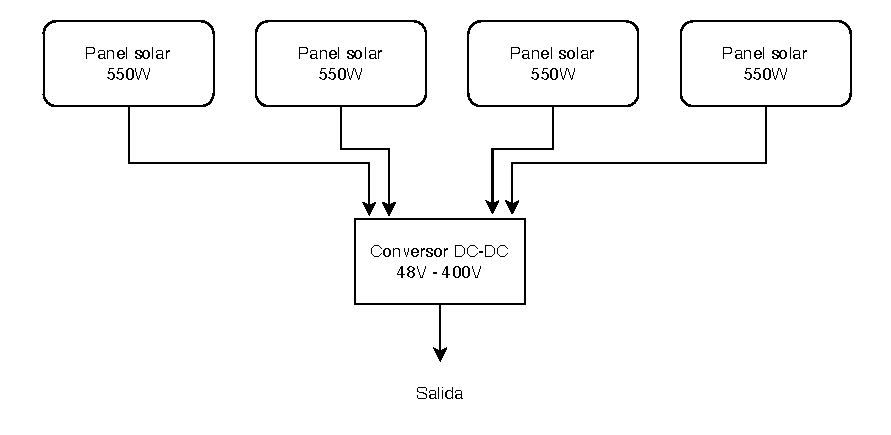
\includegraphics[width=0.7\linewidth]{img/diagramaUnConversor}
	\caption{Esquema general de un único conversor.}
	\label{fig:diagramaunconversor}
\end{figure}

Y, de forma global, se estaría usando algo como lo siguiente.

\begin{figure}
	\centering
	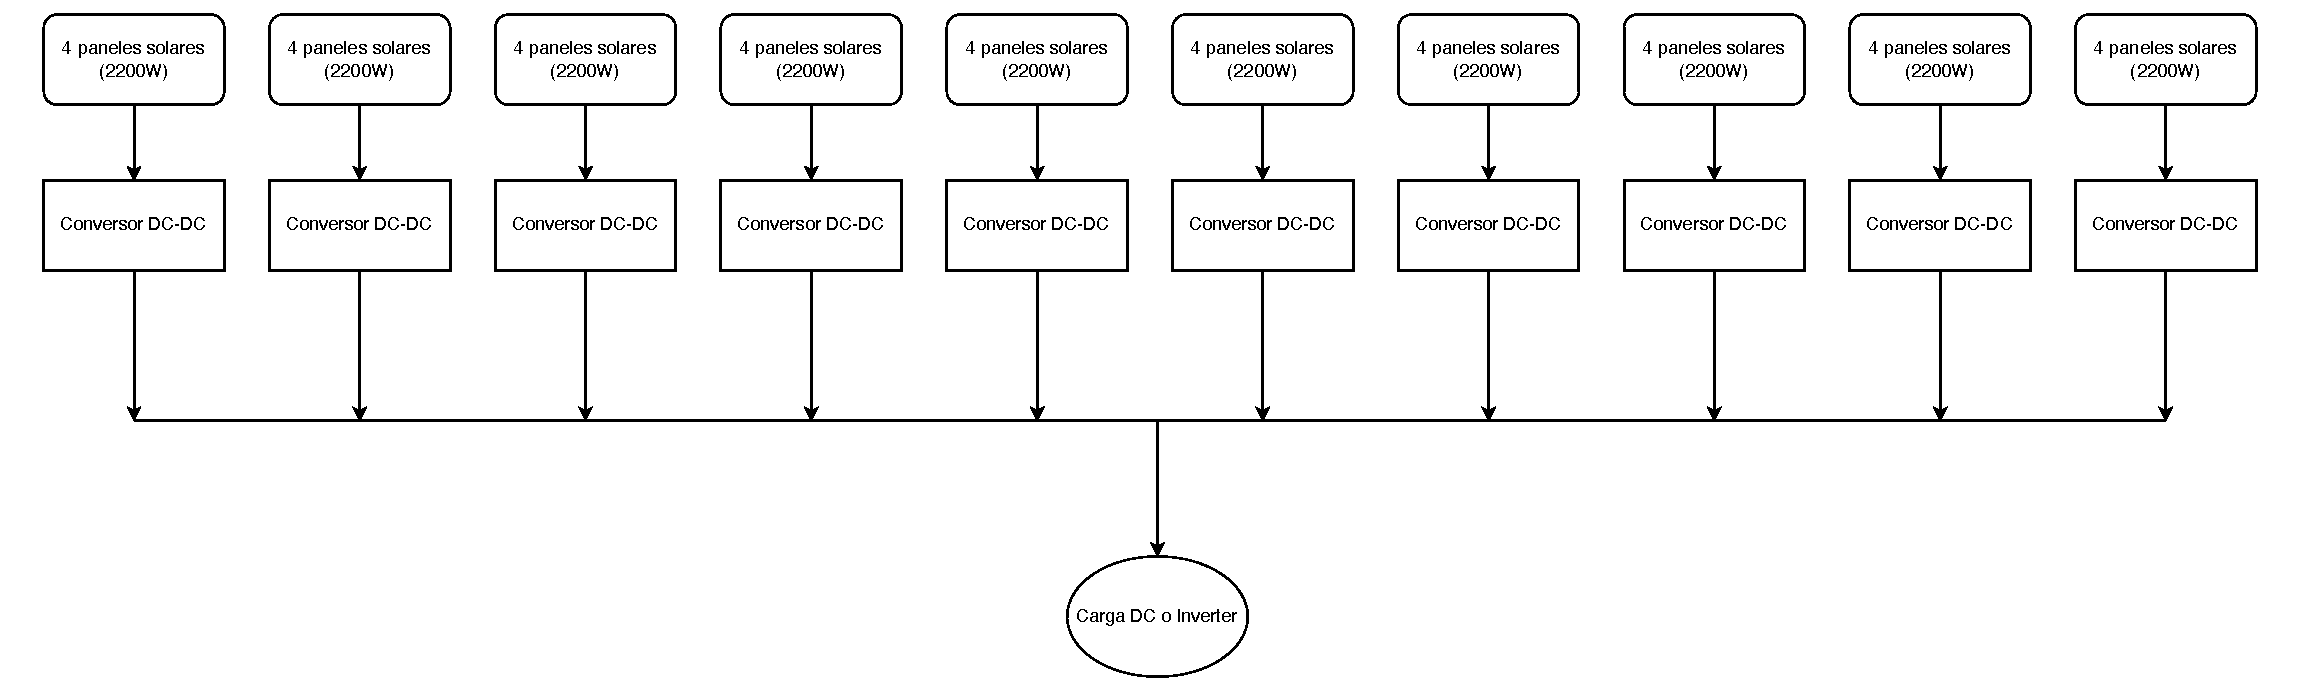
\includegraphics[width=1\linewidth]{img/diagramaTotalConversores}
	\caption{Esquema de conexión final.}
	\label{fig:diagramatotalconversores}
\end{figure}

En este circuito convertidor por diseñar, no se utilizará una técnica de modulación de ZVS, por lo que no es necesario calcular un inductor $L_{LKp}$ para lograr el cruce por cero en un determinado instante. Esto es por la razón de que la alimentación de entrada es constante, y no será necesario aplicar variaciones en el ciclo de trabajo de las señales de disparo de las llaves $S_U$ y $S_L$.


\subsection{Características deseadas}

Se diseña cada conversor con las siguientes características:

\begin{itemize}
	\item $V_{in}=48V$
	\item $P_{out}=1600W$
	\item $V_{out}=400V$
	\item $I_{out(max)}=4A$
	\item $\eta =0.9$
	\item $D=0.5$
	\item $f_s=50kHz$
\end{itemize}

\subsection{Relación de transformación}

Se parte del hecho de que:

$$
V_{out}=\frac{n\cdot V_{in}}{1-D}
$$

De donde se obtiene:

$$
n=\frac{V_{out}\cdot (1-D)}{V_{in}}=\frac{400V\cdot (1-0.5)}{48V}\approx 4.17
$$

Se eleva esa relación a $4.4$, con el fin de obtener un margen para pérdidas en los conductores, transformador, e incluso dispositivos como los diodos. Puede verse en la última expresión utilizada el funcionamiento del circuito doblador de tensión aplicado a la salida, resultante de la combinación de diodos y capacitores.

\subsection{Inductor de entrada}

Se parte de la potencia de entrada:

$$
P_{in}=\frac{1600W}{0.9}=1777.77W
$$

Entonces, la corriente de entrada será:

$$
I_{in} = \frac{P_{in}}{V_{in}}=\frac{1777.78W}{48V}=37.04A
$$

Asumiendo un ripple máximo de $20\%$, entonces se tiene:

$$
\Delta I_{in} = 0.2\cdot I_{in}=0.2\cdot 37.04 A = 7.41A
$$

Finalmente:

$$
L_{in}=\frac{V_{in}\cdot D}{f_s \cdot \Delta I_{in}}=\frac{48V\cdot 0.5}{50kHz\cdot 7.41A}=64.78 \mu H
$$

\subsection{Capacitores de entrada}

Se parte de la expresión siguiente:

$$
\frac{\Delta V}{V}=\frac{D}{R \cdot C \cdot f_s}\Rightarrow C=\frac{D}{R \cdot f_s \cdot \frac{\Delta V}{V}}
$$

En donde:

$$
R=\frac{V_{CU}+V_{CL}}{P_{out}}=\frac{V_{in}^2}{P_{out}}=\frac{(48V)^2}{1600W}=1.44\Omega
$$

Si se fija un rippple de $2\%$, entonces se tiene:

$$
C=\frac{D}{R \cdot f_s \cdot \frac{\Delta V}{V}} = \frac{0.5}{1.44 \Omega \cdot 50kHz \cdot 0.02 }=347.2 \mu F
$$

Pero, como los capacitores están en serie:

$$
C_L=C_U=2C \approx 700 \mu F
$$

\subsection{Capacitores de filtro a la salida}

Se usa la misma expresión que para la capacitancia de entrada:

$$
C=\frac{D}{R_{out} \cdot f_s \cdot \frac{\Delta V}{V}}
$$

En donde:

$$
R_{out}=\frac{V_{out}}{I_{out}}=\frac{400V}{4A}=100 \Omega
$$

Manteniendo constante la especificación de ripple de tensión:

$$
C=\frac{D}{R_{out} \cdot f_s \cdot \frac{\Delta V}{V}}=\frac{0.5}{100\Omega \cdot 50kHz \cdot 0.02}=5 \mu F
$$

Nuevamente, se tienen capacitores en serie, por lo que:

$$
C_{RU}=C_{RL}=10 \mu F
$$

\subsection{Ciclos de trabajo de las señales}

Como fue mencionado anteriormente, se trabajará con un ciclo de trabajo de $0.5$. Este valor es aplicable al disparo de la llave $S_U$, sin embargo, para la llave $S_L$ es necesario que su $D$ sea menor a $0.5$, de modo de evitar problemas de cortocircuito. Se decide por utilizar un tiempo muerto de $0.5 \mu s$, lo que implica que la segunda llave debería estar encendida por un período de tiempo calculado como:

$$
t_{on(L)}=0.5\cdot T_s-2 \cdot 0.5 \mu s=9\mu s
$$

Que es equivalente a un ciclo de trabajo de $0.45$, en donde el delay de fase, es de $10 \mu s+0.5 \mu s=10.5 \mu s$.

\subsection{Red Snubber RCD}

Se implementa una pequeña red snubber RCD para los dispositivos IGBT, la misma está compuesta por un capacitor de $1 \ nF$ y un resistor de $1 \ k \Omega$.


\clearpage


\section{Simulación}

Para esta simulación se trabaja con PLECS (Plexim), en su versión más reciente (4.8) corriendo en MacOS Sonoma. Se trabaja con la versión standalone del programa y se corren las simulaciones mediante localhost con un script de Python.

\subsection{Circuito implementado}

Para una simulación con componentes ideales, se trabaja con el software de simulación PLECS, en su versión 4.8 (corriendo en sistema operativo MacOS). Se parte del siguiente esquemático a implementar. 

\begin{figure}
	\centering
	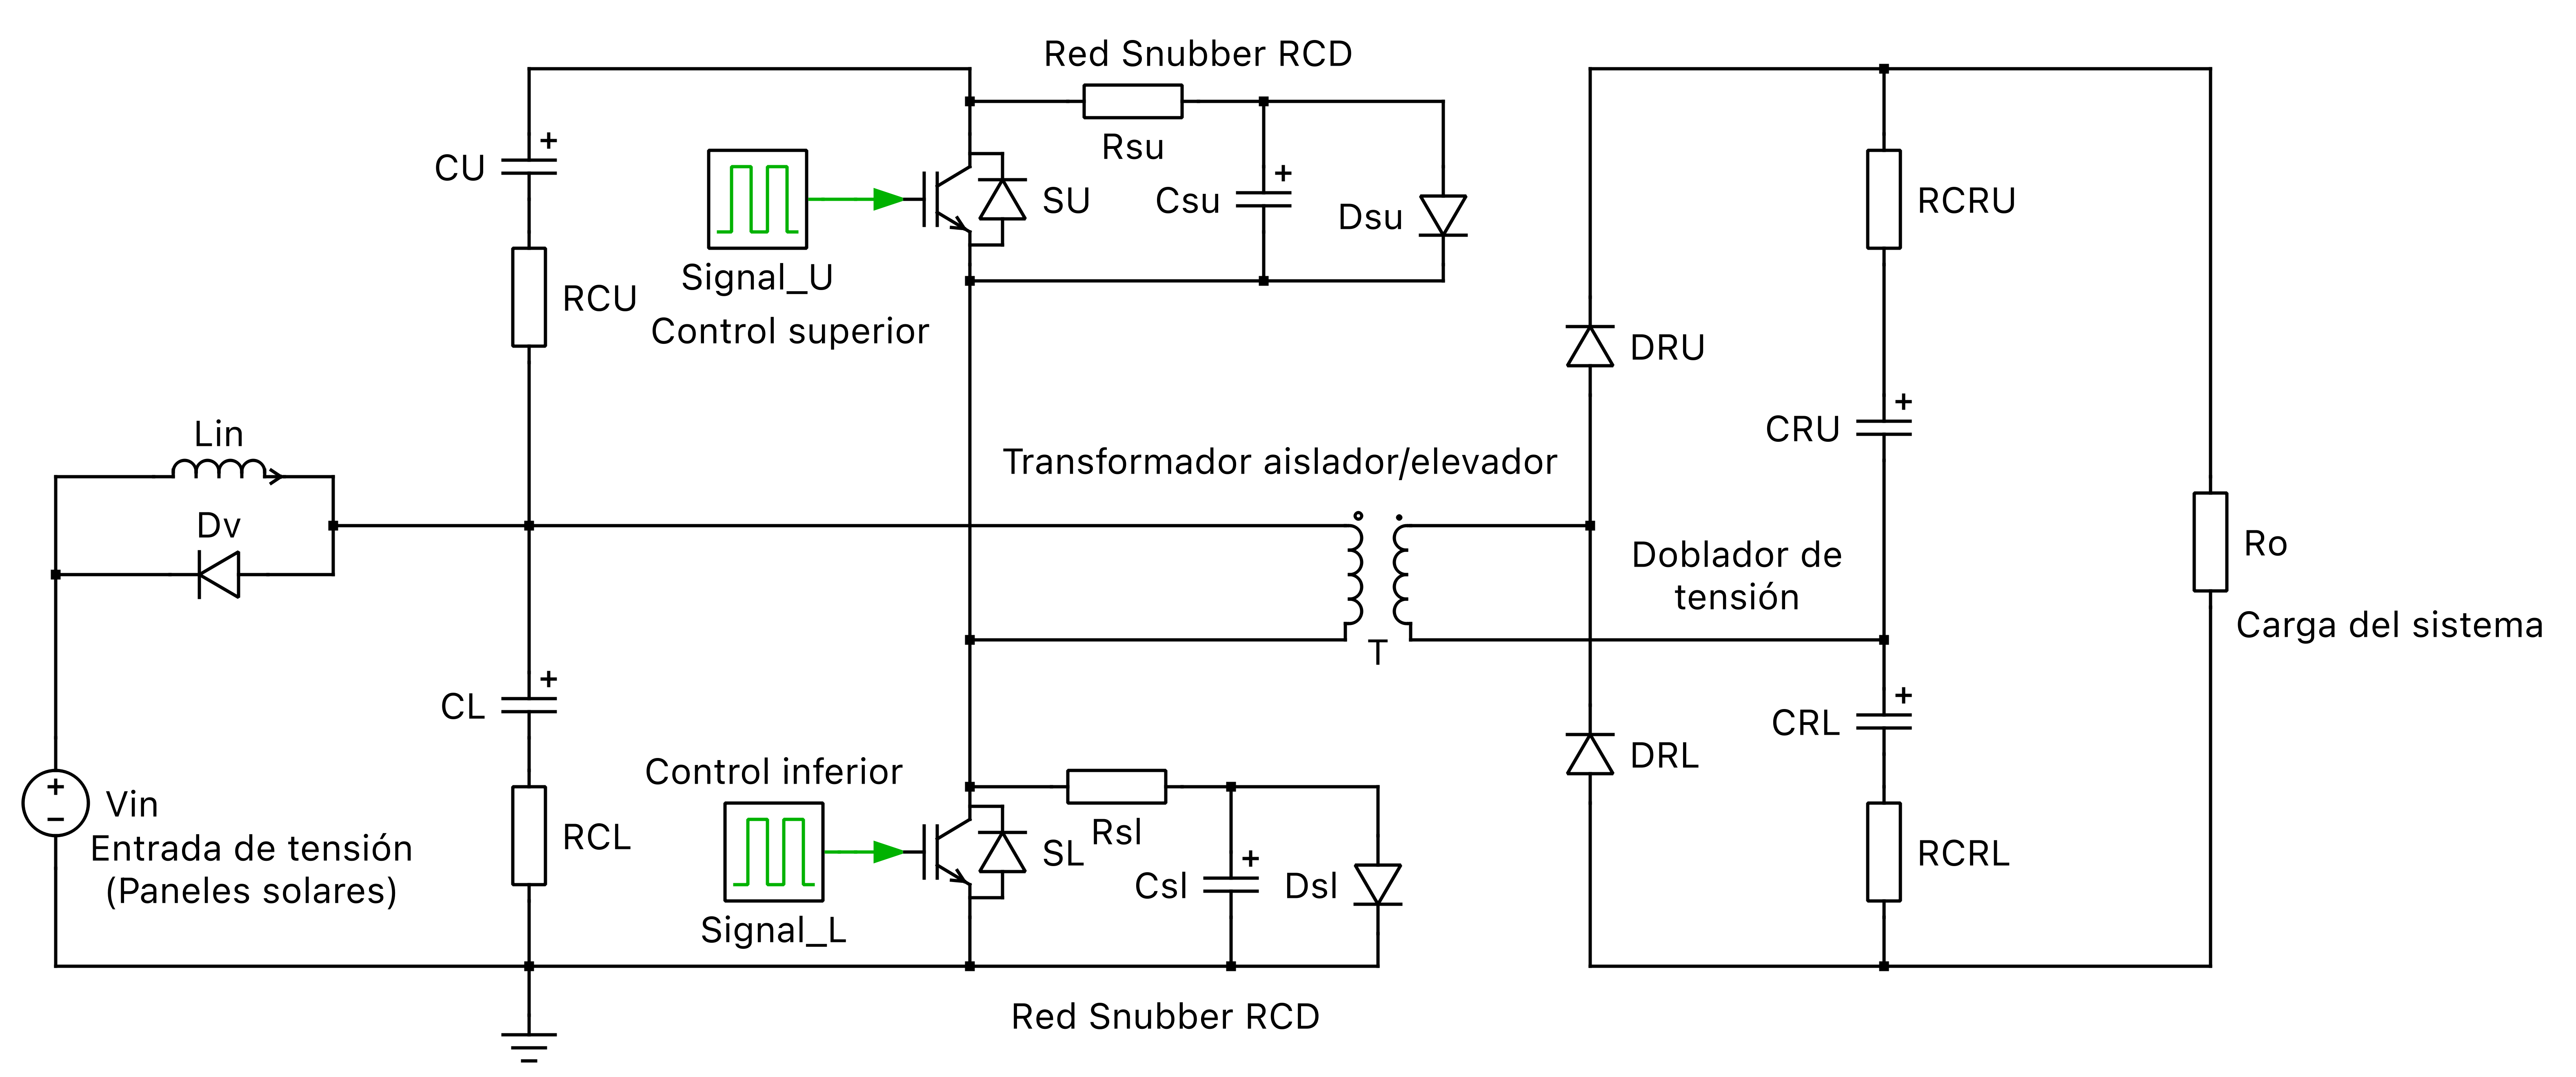
\includegraphics[width=1\linewidth]{img/schematic}
	\caption{Esquemático del circuito implementado en PLECS.}
	\label{fig:schematic}
\end{figure}

Puede verse algunos cambios en el circuito de alimentación, se mencionan a continuación:

\begin{enumerate}
	\item Se agrega un diodo volante a la inductancia $L_{in}$.
	\item Resistores en serie con los capacitores del sistema.
\end{enumerate}

El diodo volante conectado al inductor $L_{in}$ sirve para proteger el circuito de entrada de una realimentación negativa a la fuente en el caso de que se encuentre operando el circuito sin carga, ya que prácticamente se está teniendo una carga RL.

Los resistores en serie con cada uno de los capacitores se usan a modo de protección contra saltos discretos de los valores de tensión o corriente en los capacitores. Esto es por la forma en que el simulador PLECS interpreta los modelos, en la página web del software recomiendan una resistencia de pequeño valor en serie para poder mitigar estos efectos. Para todos los casos se usan resistores de $1 \ m\Omega$.

\subsection{Formas de onda}

\subsubsection{Señales de disparo}

Las formas de onda de disparo de los transistores IGBT son las que se muestran en la figura 14. Allí es posible apreciar el tiempo muerto simétrico existente entre las conmutaciones de ambos dispositivos de switching.

\begin{figure}
	\centering
	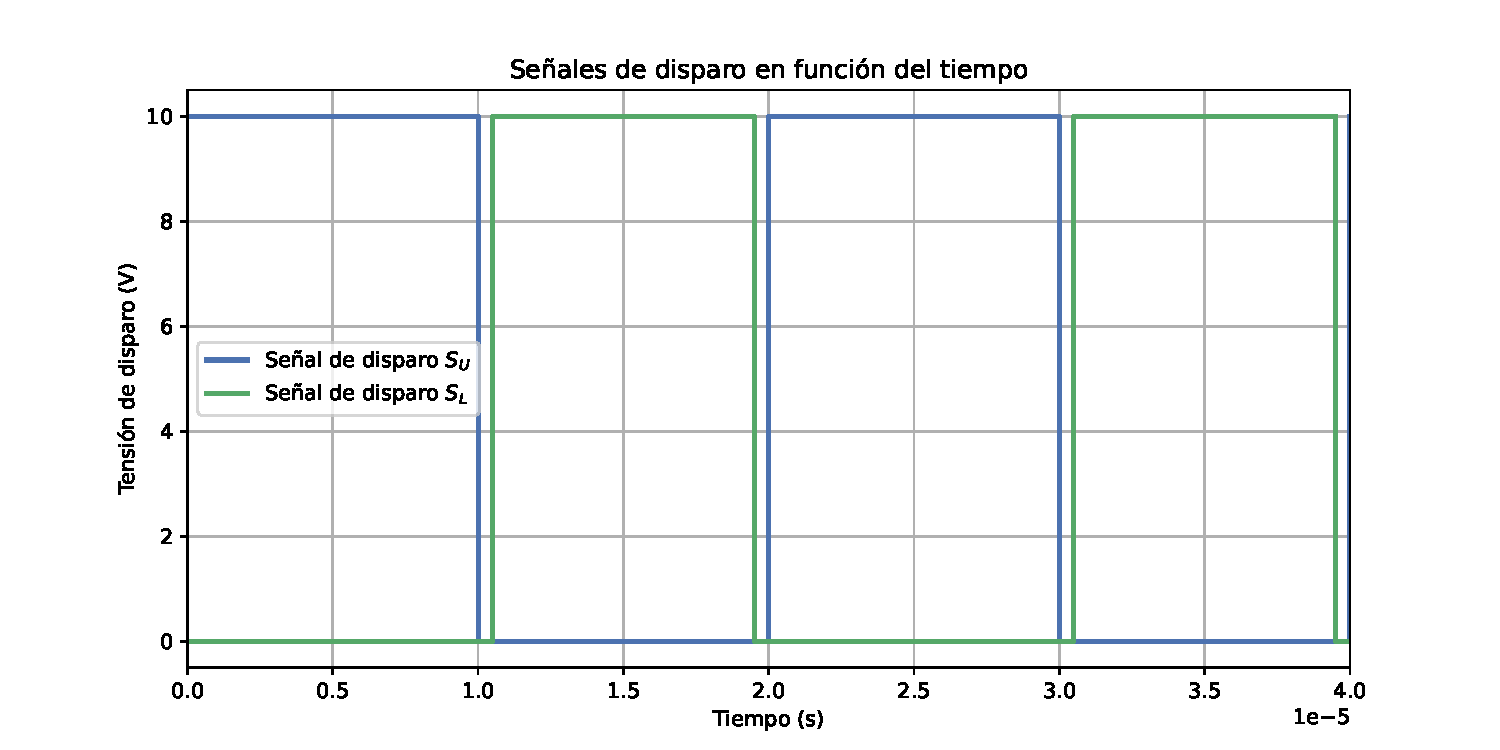
\includegraphics[width=1\linewidth]{img/disparo}
	\caption{Señales de disparo de los IGBT.}
	\label{fig:disparo}
\end{figure}

\subsubsection{Señales de salida}

Ahora, para la tensión y corriente de salida, se tienen las siguientes formas de onda. Vale aclarar que se toma como referencia la salida de mayor potencia del diseño. Eso se logra con un resistor, como fue calculado anteriormente, de $100 \ \Omega$. En la figura se puede apreciar ese pequeño ripple, así como también que el tiempo de establecimiento de la señal es muy pequeño, existiendo un sobrepasamiento de $21 \ V$, es decir, $5\%$.

\begin{figure}
	\centering
	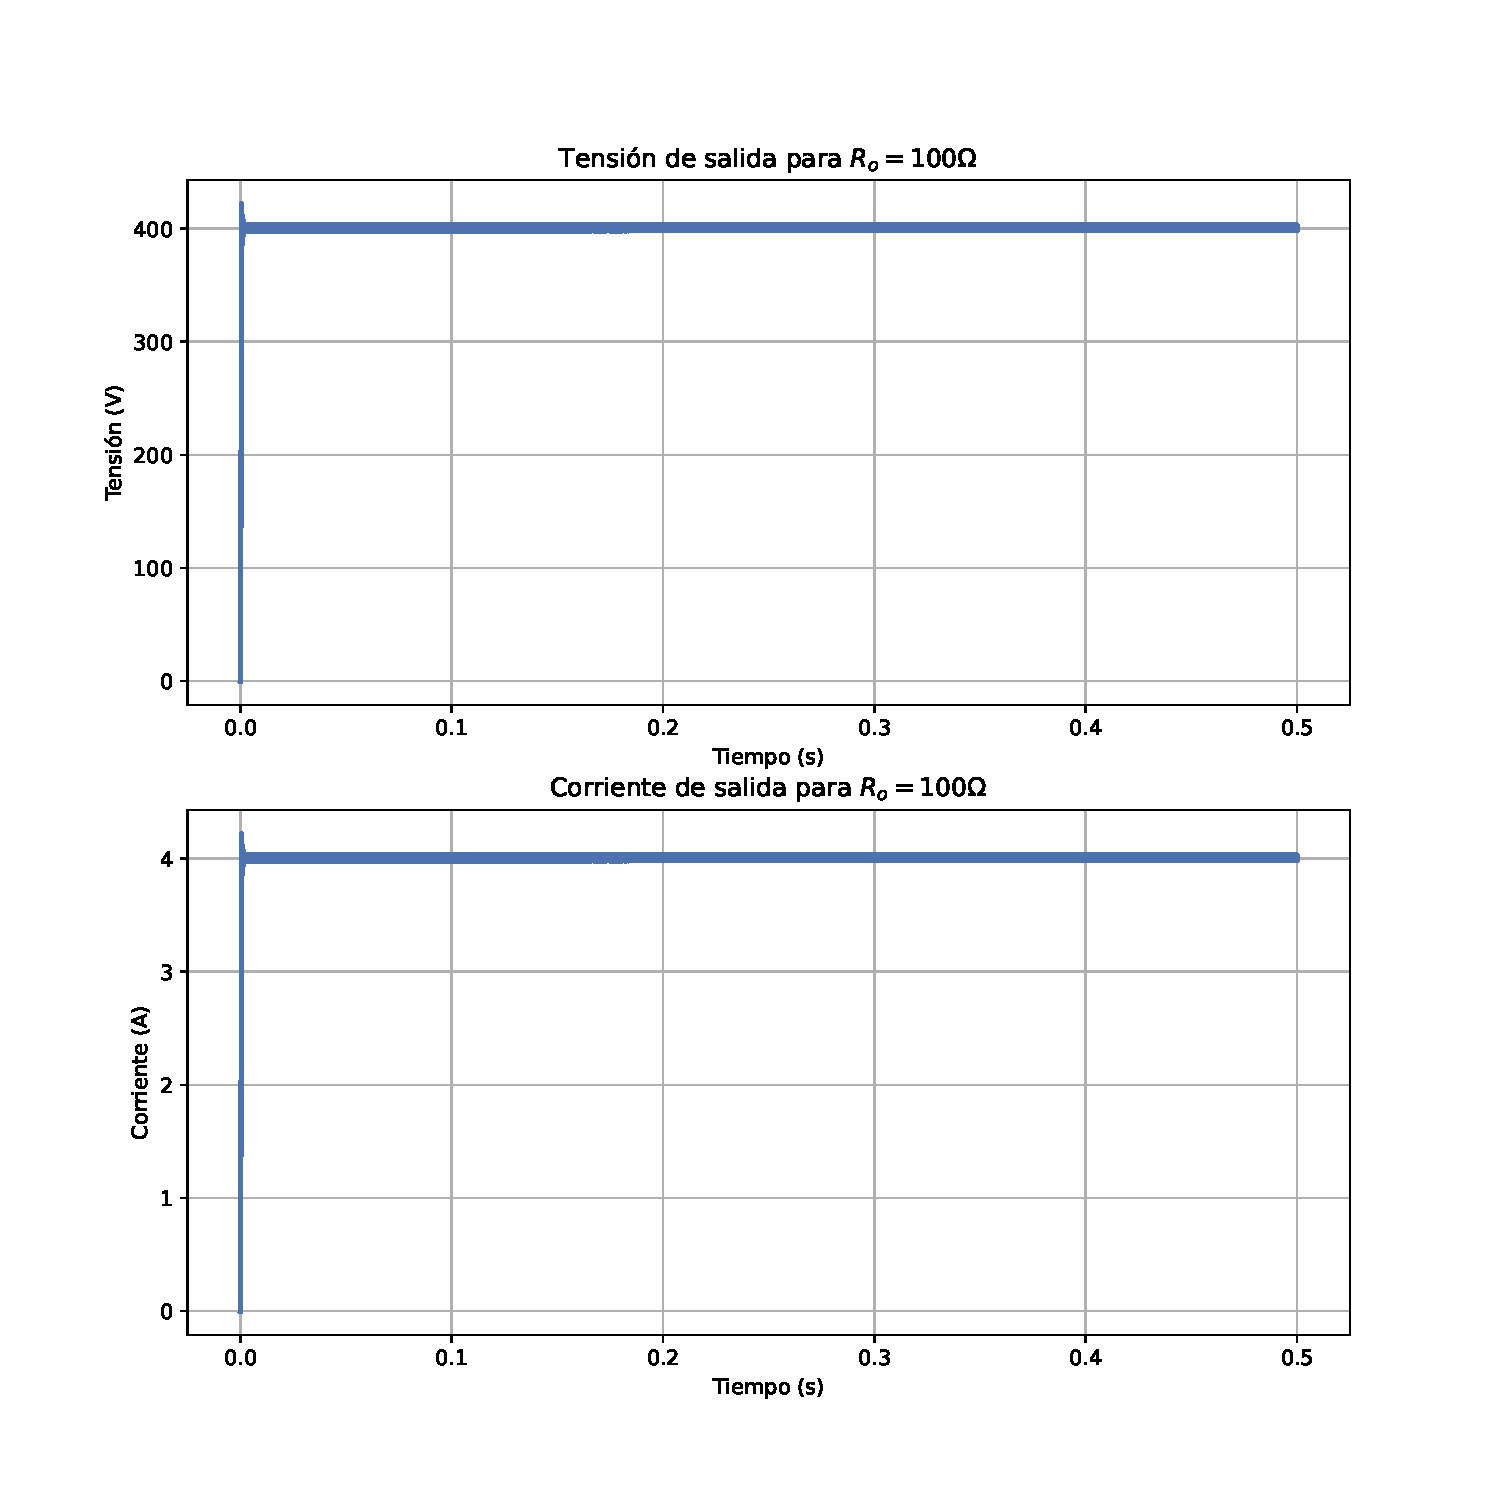
\includegraphics[width=1\linewidth]{img/salida_40}
	\caption{Señales de salida para máxima carga.}
	\label{fig:salida40}
\end{figure}

De forma de apreciar mejor el transitorio, se ilustra a continuación, en la figura 16 el mismo en la onda de tensión. Vale la pena destacar que para ambas señales mostradas en la figura 15 la forma es la misma, cambia la escala por tratarse de diferentes magnitudes eléctricas.

\begin{figure}
	\centering
	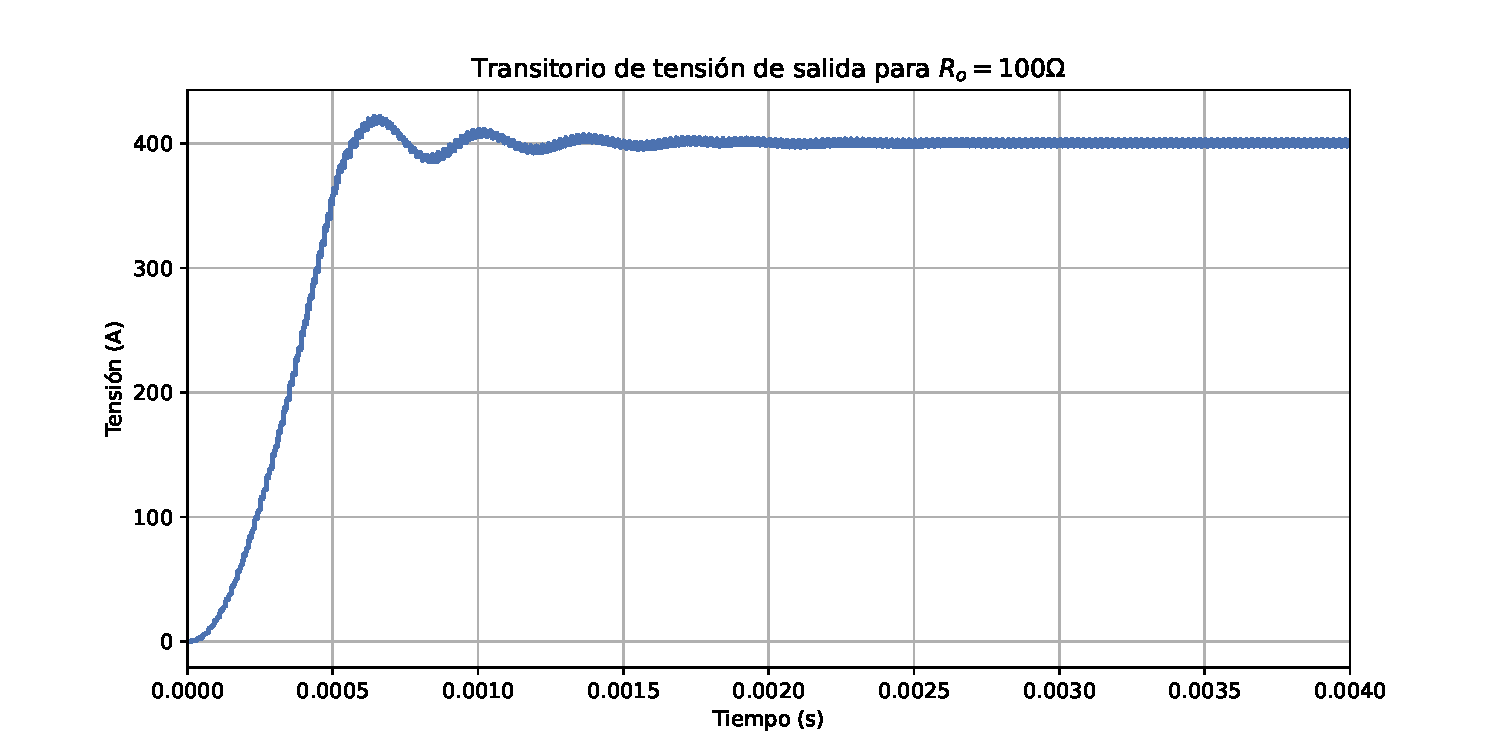
\includegraphics[width=1\linewidth]{img/transitorio}
	\caption{Transitorio de la señal de salida.}
	\label{fig:transitorio}
\end{figure}

El tiempo de establecimiento, medido con el programa de simulación y Python es de aproximadamente $0.35 \ ms$, es decir, se trata de un sistema rápido para la mayoría de aplicaciones.


Ahora, la señal de potencia de la salida del convertidor para la carga máxima se ve a continuación.

\begin{figure}
	\centering
	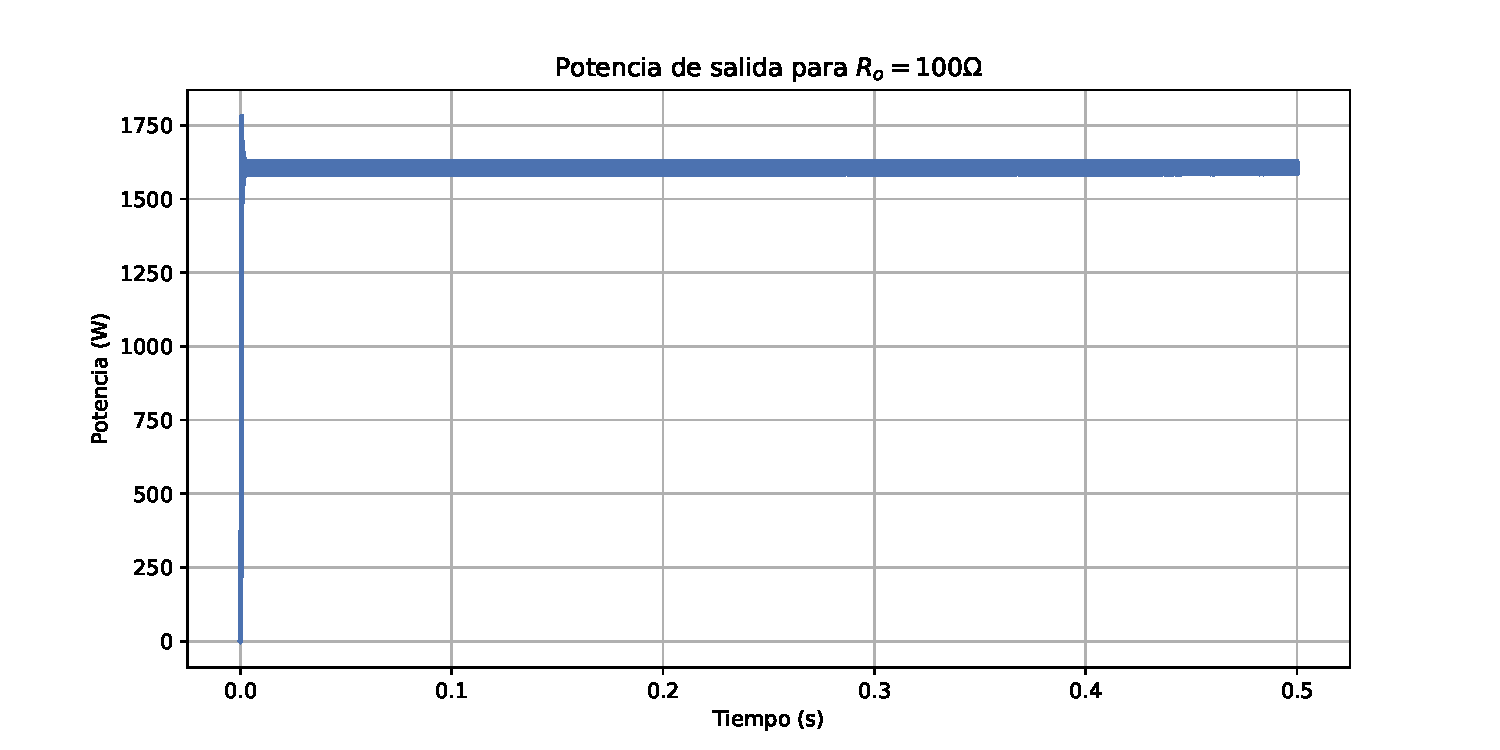
\includegraphics[width=1\linewidth]{img/potencia}
	\caption{Potencia de salida para máxima carga.}
	\label{fig:potencia}
\end{figure}

\subsubsection{Señales en los IGBTs}

Las formas de onda por sobre los transistores IGBT se muestran a continuación, se encuentra una tensión máxima de colector emisor de $92 \ V$, y una corriente de colector eficaz de $115.16 \ A$, valores que posteriormente serán utilizados para la selección del componente.

\begin{figure}
	\centering
	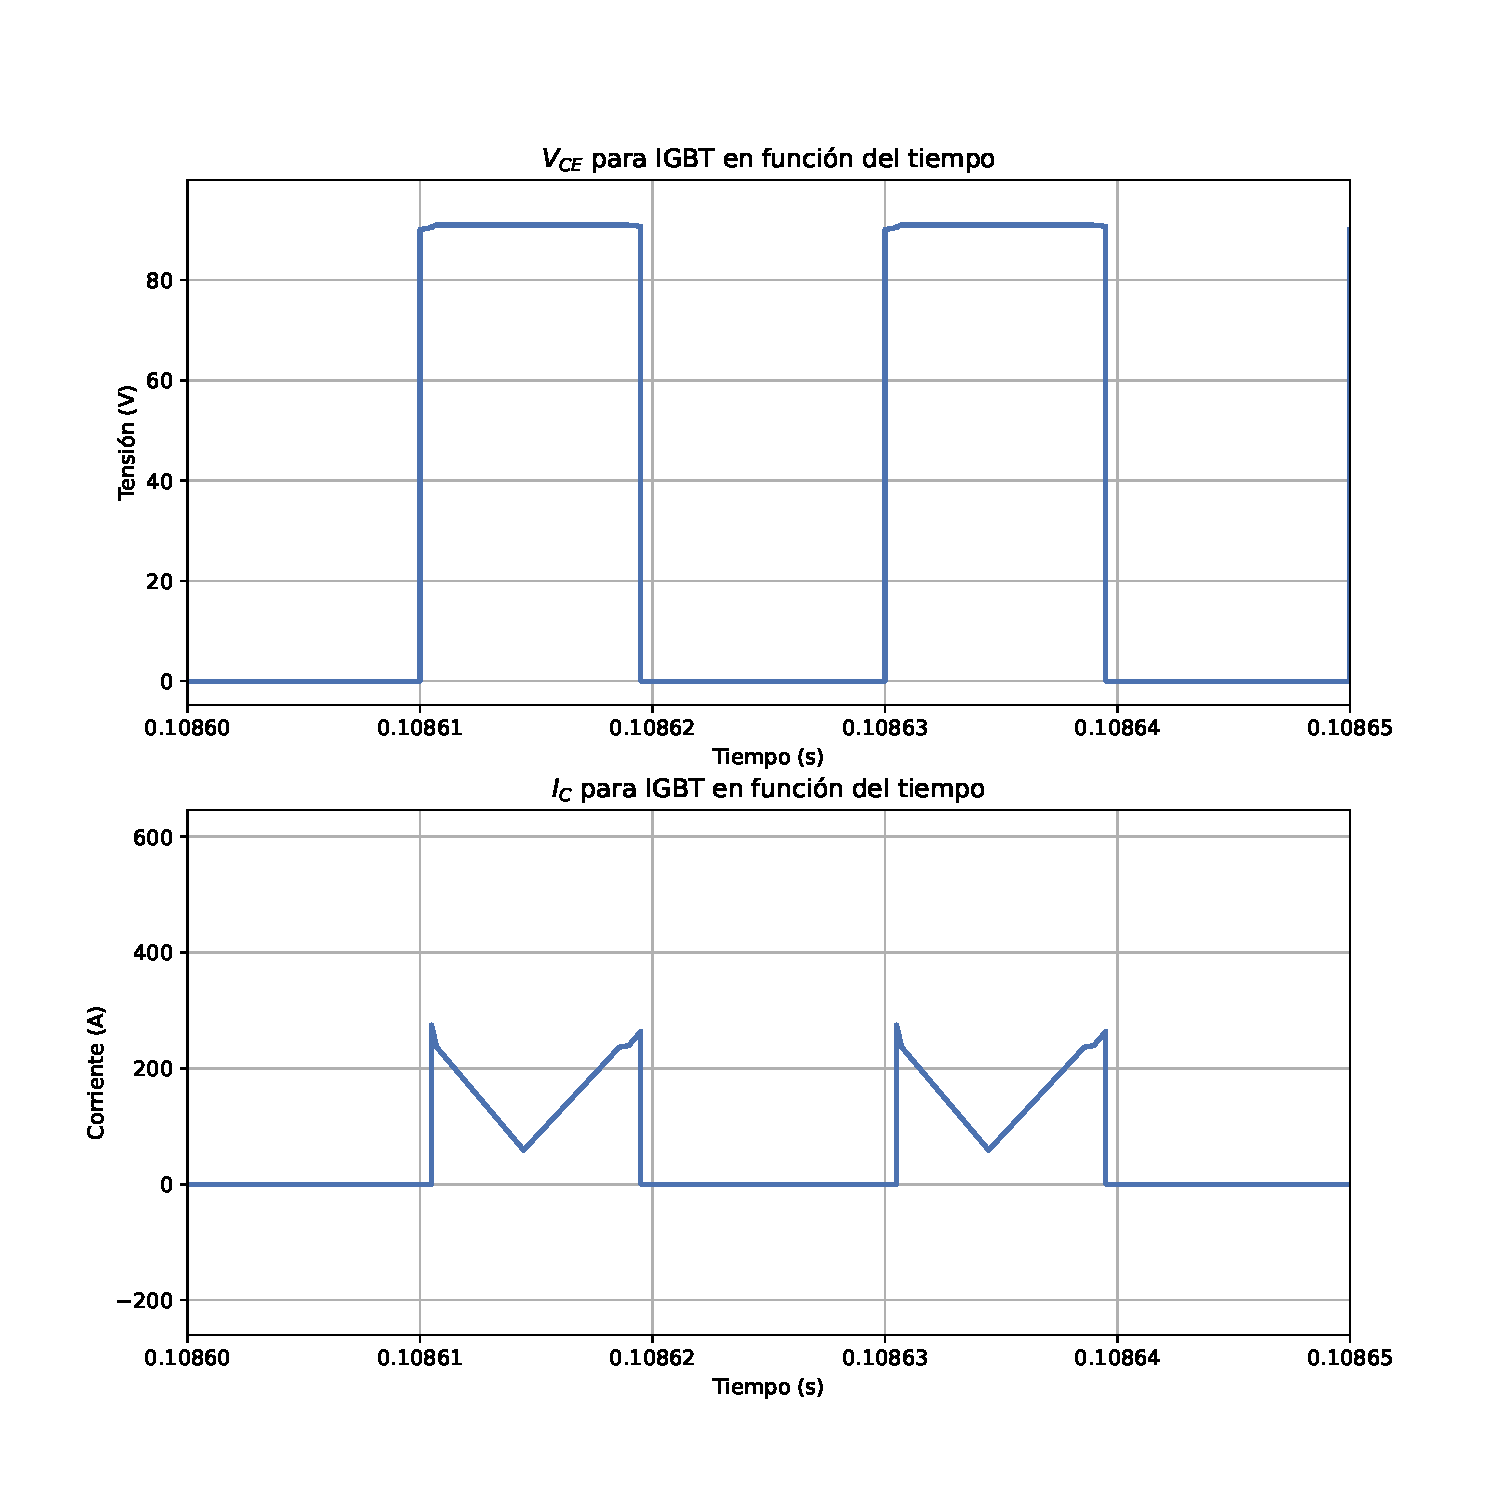
\includegraphics[width=1\linewidth]{img/signal_IGBT}
	\caption{Señales de tensión y corriente en los IGBT implementados.}
	\label{fig:signaligbt}
\end{figure}

\subsubsection{Señales en el transformador}

Las tensiones en los devanados del transformador se pueden apreciar en la siguiente figura.

\begin{figure}
	\centering
	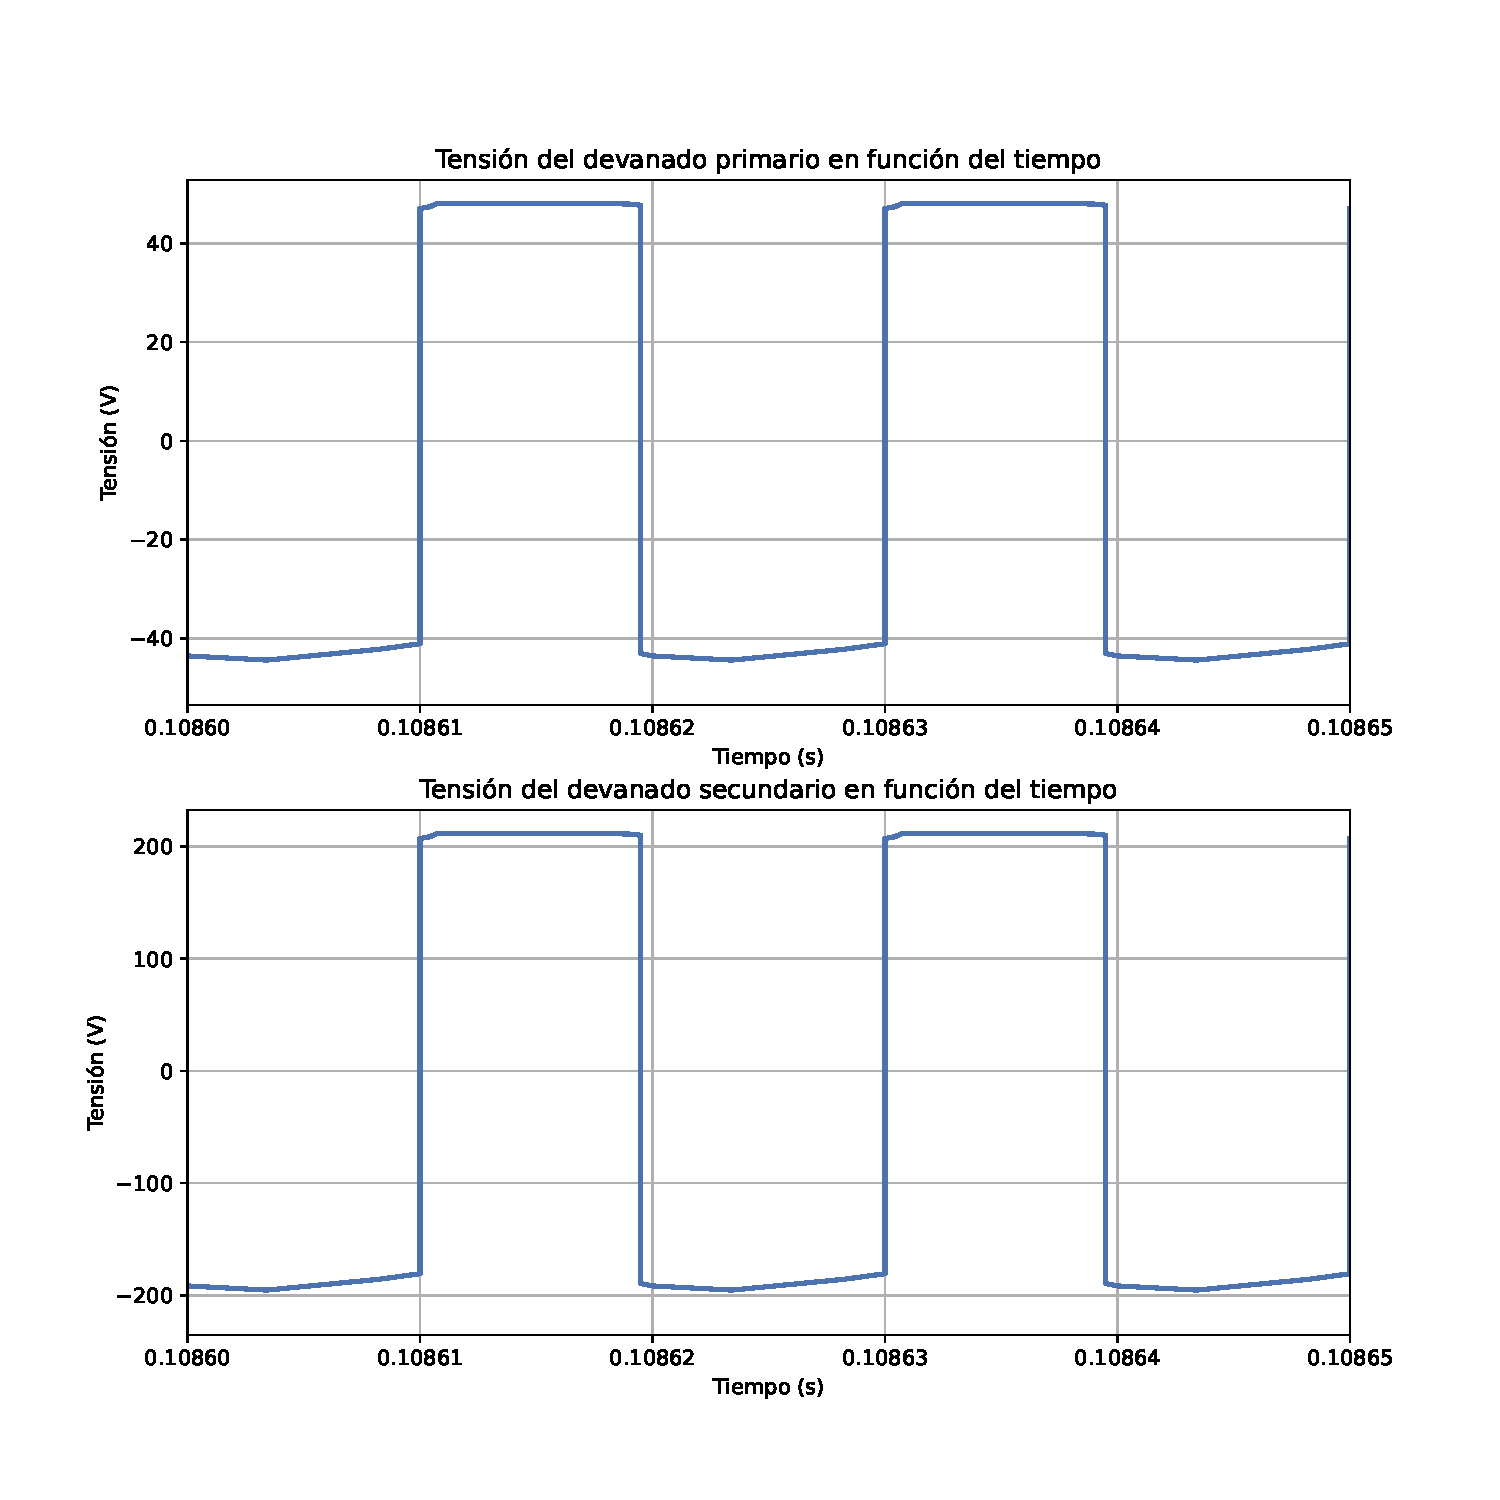
\includegraphics[width=1\linewidth]{../../tensiones_transformador}
	\caption{Tensiones en los devanados del transformador.}
	\label{fig:tensionestransformador}
\end{figure}

Mientras que a continuación se muestran los valores de corriente en el mismo transformador elevador del circuito implementado.

\begin{figure}
	\centering
	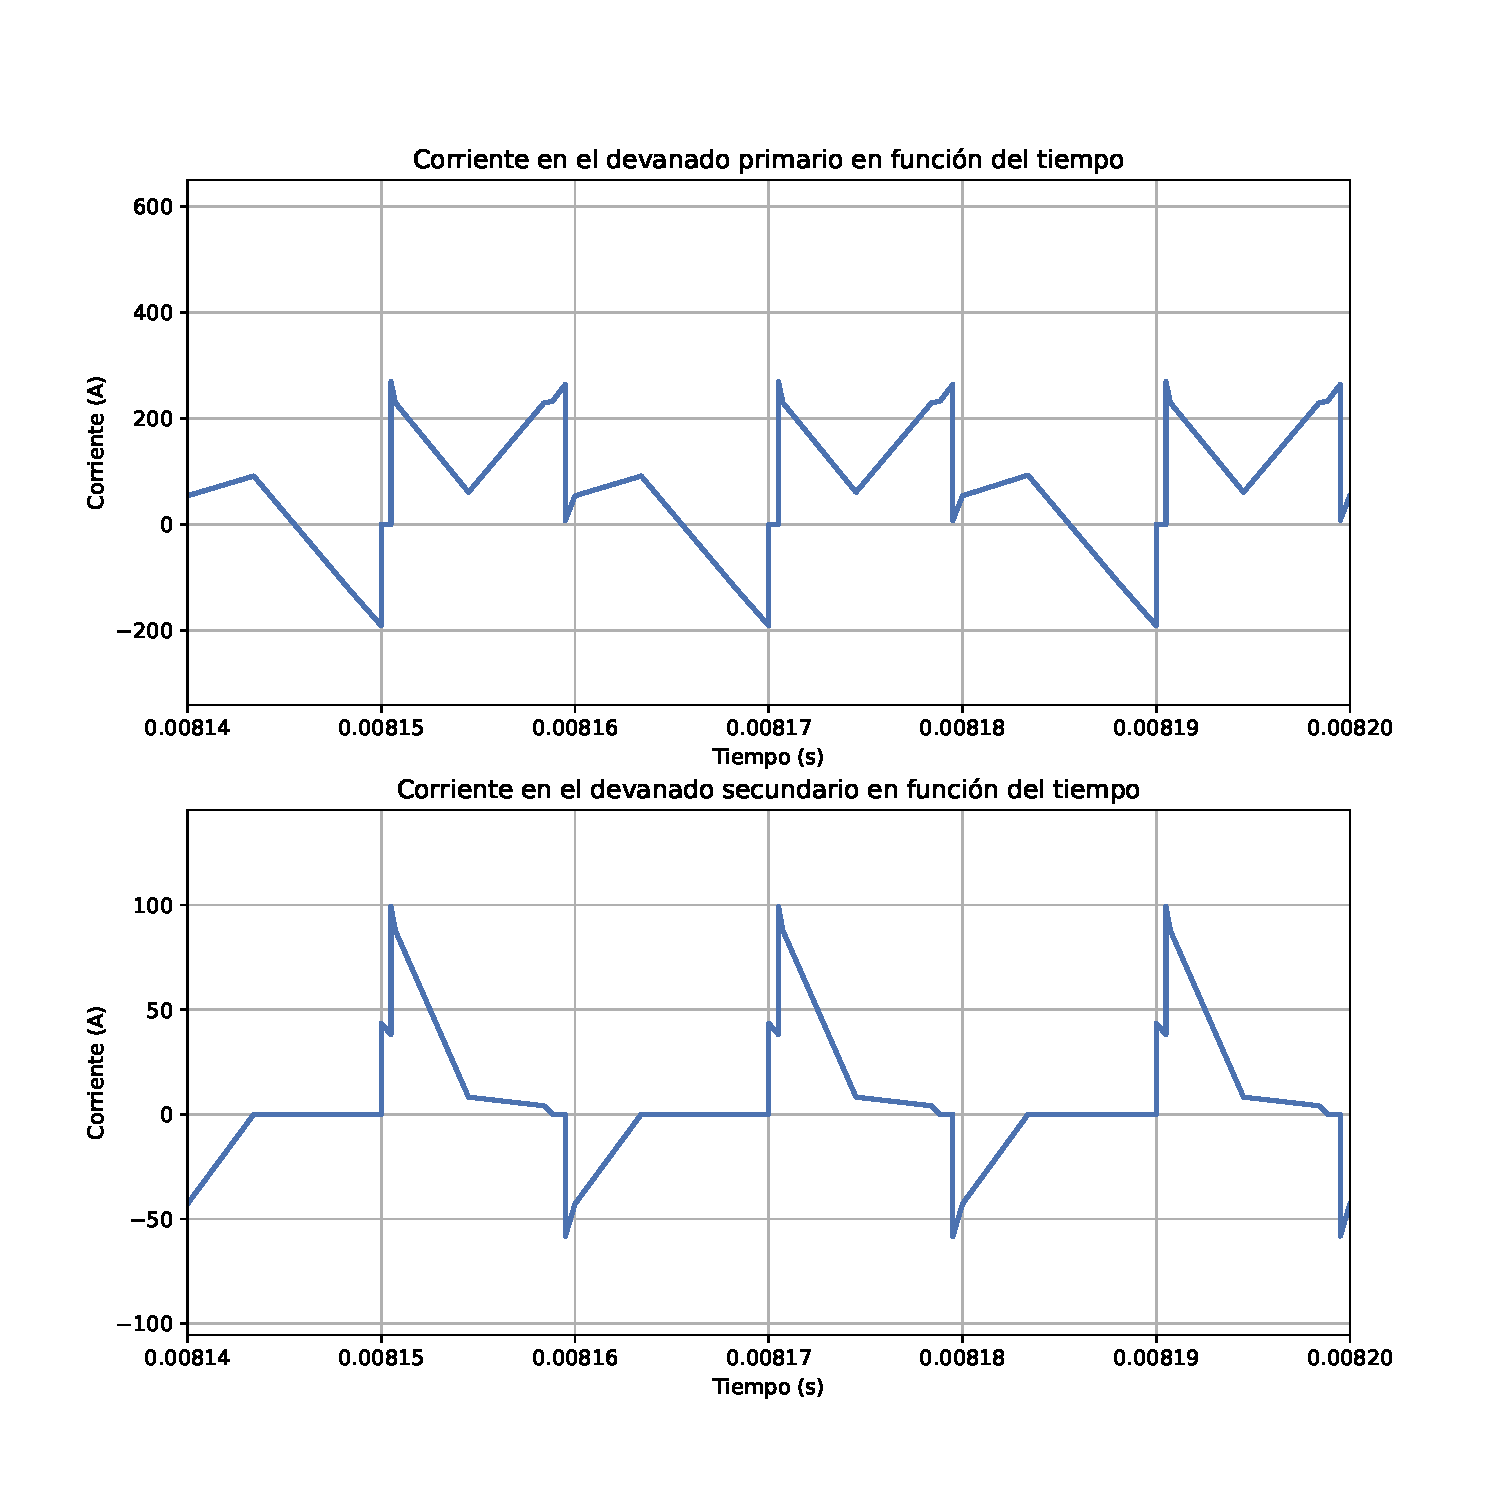
\includegraphics[width=1\linewidth]{../../corrientes_transformador}
	\caption{Corrientes en los devanados del transformador.}
	\label{fig:corrientestransformador}
\end{figure}


\clearpage

\section{Selección de componentes}

\subsection{Criterios a adoptar}

Para la selección de diodos, se toman en cuenta los dos siguientes parámetros:

\begin{itemize}
	\item Tensión inversa repetitiva máxima $V_{RRM}$
	\item Corriente promedio $I_{F(av)}$
\end{itemize}

Para los IGBTs:

\begin{itemize}
	\item Tensión máxima en colector-emisor $V_{CE(max)}$
	\item Corriente eficaz por el colector $I_{C(rms)}$
	\item Tiempo de recuperación inversa $t_{rr}$
\end{itemize}

Y, para los capacitores se tiene en cuenta la máxima tensión a soportar.

Finalmente, para los valores de tensión encontrados como parámetro, se usa un factor de seguridad de $2.5$, mientras que para valores de corriente el factor será de $1.3$.

\subsection{Selección del IGBT}

Para seleccionar el IGBT, se tienen los siguientes parámetros:

\begin{itemize}
	\item $I_{C(rms)}=117 A$
	\item $V_{CE(max)} = 92 V$
	\item $T_s=20\mu s$
\end{itemize}

Lo que resulta aplicando factores de seguridad, y proponiendo que el tiempo de recuperación inversa sea menor al $10\%$ del período de conmutación:

\begin{itemize}
	\item $I_C(=152.1A$
	\item $V_{BR} = 230V$
	\item $t_{rr} = 2 \mu s$
\end{itemize}

Se opta por utilizar el IGBT modelo IXSX 80N60B , de la marca IXYS. 

\begin{table}[h]
	\centering
	\begin{tabular}{|c|c|c|}
		\hline
		\textbf{Símbolo} & \textbf{Condiciones de prueba} & \textbf{Valores máximos} \\ \hline
		VCES & TJ = 25°C to 150C & 600 V \\ \hline
		VCGR & TJ = 25°C to 150C; RGS = 1 MΩ & 600 V \\ \hline
		VGES & Continuous & ±20 V \\ \hline
		VGEM & Transient & ±30 V \\ \hline
		IC25 & TC = 25C (silicon chip capability) & 160 A \\ \hline
		IC90 & TC = 90C (silicon chip capability) & 80 A \\ \hline
		IL(RMS) & TC = 90C (silicon chip capability) & 75 A \\ \hline
		ICM & TC = 25C, 1 ms & 300 A \\ \hline
		SSOA (RBSOA) & VGE = 15 V, TVJ = 125C, RG = 5 Ω & ICM = 160 A \\
		& Clamped inductive load @ 0.8 VCES & \\ \hline
		tsc & VGE = 15 V, VCE = 0.6 VCES, TJ = 125°C & 10 µs \\ \hline
		SCSOA & RG = 5 Ω, non-repetitive & \\ \hline
		PC & TC = 25°C & 500 W \\ \hline
		TJ &  & -55 ... +150 C \\ \hline
		TJM &  & 150 C \\ \hline
		Tstg &  & -55 ... +150 C \\ \hline
		TL & 1.6 mm (0.063 in.) from case for 10 s & 300 C \\ \hline
		Md & Mounting torque TO-264 & 0.4/6 Nm/lb.in. \\ \hline
		td(on) &  & 60 ns \\ \hline
		tri &  & 45 ns \\ \hline
		td(off) &  & 140 280 ns \\ \hline
		tfi &  & 180 280 ns \\ \hline
		Eoff &  & 4.2 7.0 mJ \\ \hline
	\end{tabular}
	\caption{Características del IGBT seleccionado.}
	\label{tab:test_conditions}
\end{table}
\clearpage

\subsection{Selección de diodos}

\subsubsection{Diodos de snubber}

\begin{figure}
	\centering
	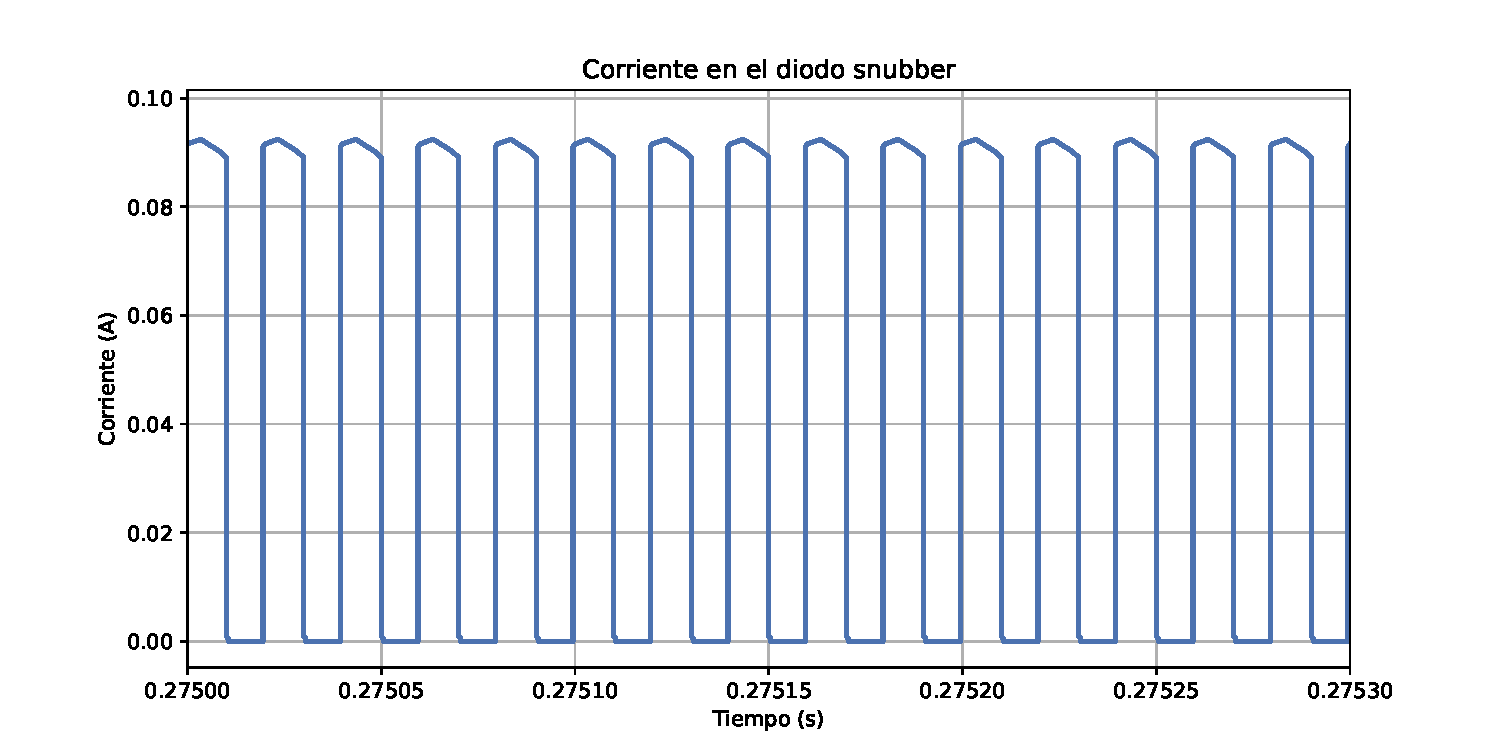
\includegraphics[width=1\linewidth]{img/diodo_snubber}
	\caption{Corriente en el diodo de snubber}
	\label{fig:diodosnubber}
\end{figure}


De la simulación, se obtiene como valor medio de corriente por los diodos $0.047 \ A$, por lo que, afectando ese valor por el factor de seguridad propuesto, se obtiene como parámetro de selección $I_{F(av)}=0.06 \ A$, y, como tensión inversa repetitiva máxima, se usa un valor de $92 \ V$, siendo este el que soporta como máximo cada IGBT, obteniéndose así para seleccionar $V_{RRM}=230 \ V$. 

Con los parámetro mencionados, se selecciona el diodo 1N4004, fabricado por Vishay, cuyas características se adjuntan a continuación.

\begin{table}[h]
		\begin{tabular}{|l|l|}
			\hline
			\textbf{Parámetro} & \textbf{Valores} \\
			\hline
			IF(AV) & 1.0 A \\
			\hline
			VRRM & 400 V \\
			\hline
			IFSM (8.3 ms sine-wave) & 30 A \\
			\hline
			IFSM (square wave tp = 1 ms) & 45 A \\
			\hline
			VF & 1.1 V \\
			\hline
			IR & 5.0 $\mu$A \\
			\hline
			TJ max. & 150 °C \\
			\hline
			Package & DO-41 (DO-204AL) \\
			\hline
			Circuit configuration & Single \\
			\hline
		\end{tabular}
		\caption{Características principales del diodo para snubber seleccionado.}
\end{table}

\subsubsection{Diodos de salida}

\begin{figure}
	\centering
	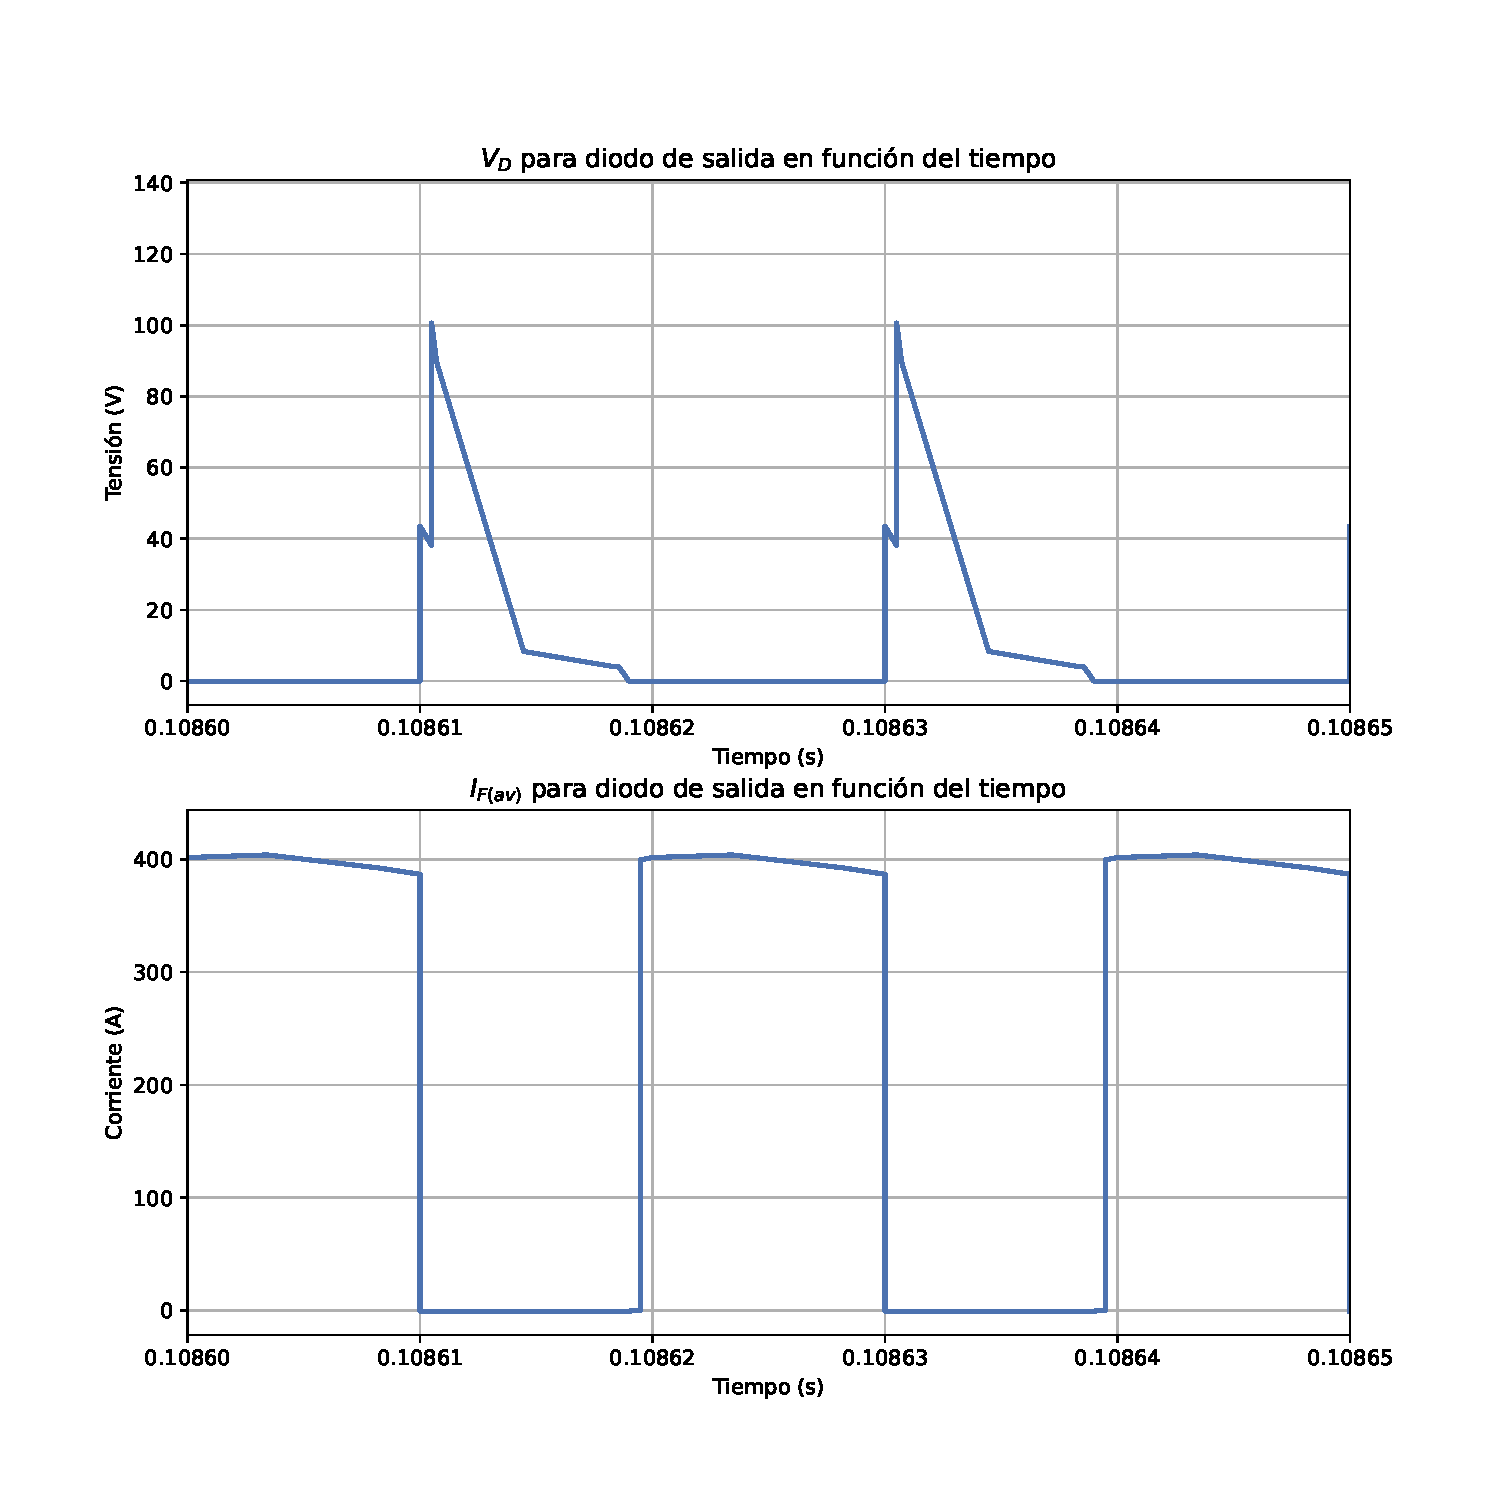
\includegraphics[width=0.8\linewidth]{img/diodo_salida}
	\caption{Señales en el diodo de salida.}
	\label{fig:diodosalida}
\end{figure}

Puede verse que el diodo no está sometido a una tensión inversa, por lo que el parámetro que queda para seleccionar es el de corriente. Se mide una corriente media de $12.54 \ A$, usando así para seleccionar $I_{F(av)}=16.3 \ A$. Se selecciona el diodo VS-20ETS16THM3 de Vishay, cuyas características principales son las siguientes:

\begin{table}[h]
	\begin{tabular}{|l|l|}
		\hline
		\textbf{Parámetro} & \textbf{Valores} \\
		\hline
		IF(AV) & 20 A \\
		\hline
		VRRM & 1600 V \\
		\hline
		IFSM  & 300 A \\
		\hline
		VF & 1.1 V \\
		\hline
		TJ max. & 150 °C \\
		\hline
		Package & 2L TO-220AC \\
		\hline
		Circuit configuration & Single \\
		\hline
	\end{tabular}
	\caption{Características principales del diodo para salida seleccionado.}
\end{table}

\subsubsection{Diodo volante para el inductor de entrada}

La corriente media por sobre ese diodo es de aproximadamente $170 \ A$, lo que implica que es necesario un valor de selección de $221 \ A$ para la corriente promedio, y, en cuanto a tensión, se verifica que la máxima repetitiva no supera los $0.5 \ V$, por lo que no existiría problema en ese caso. Se selecciona el diodo DL161-250-18 de AS Energi, que tiene un valor de $I_{F(av)} = 250 \ A$ y $V_{RRM}=800 \ V$.
\subsection{Selección de capacitores}

\subsubsection{Capacitores de entrada y snubber}

Estos capacitores están sometidos a una tensión máxima del mismo valor que la de alimentación, por lo que se usa como valor de selección $120 \ V$. 

Para la entrada, se tienen los capacitores B43416C9707A000 de la empresaTDK), los mismos son de $700 \ \mu F$ y $400 \ V$.

Para la red snubber, se selecciona el capacitor 413F1100(1)D0(2)  de la marca Kemet (Yageo company), existen en valores de $1 \ nF$, por lo que no es necesario una configuración en paralelo.

\subsubsection{Capacitores de salida}

Estos capacitores dobladores de tensión aportan cada uno una tensión de $200 \ V$, por lo que se debe verificar que soporte cada uno una tensión de $500 \ V$. Se selecciona el capacitor A10050014030 de la marca FTcap, que cuenta con exactamente las características  requeridas, así como una tolerancia de $20\%$. En la hoja de datos se menciona el uso en fuentes conmutadas como una de las aplicaciones del mismo, lo que indica que sirve para el propósito de este trabajo práctico. 





\clearpage

\section{Informes con \LaTeX}

% SUB-SECCIÓN
% Las sub-secciones se inician con \subsection, si se quiere una sub-sección
% sin número se pueden usar las funciones \subsectionanum (nuevo subtítulo sin
% numeración) o la función \subsectionanumnoi para crear el mismo subtítulo sin
% numerar y sin aparecer en el índice
\subsection{Una breve introducción}
	
	Este es un párrafo, puede contener múltiples \quotes{Expresiones} así como fórmulas o referencias\footnote{Las referencias se hacen utilizando la expresión \texttt{\textbackslash label}\{etiqueta\}.} como \eqref{eqn:identidad-imposible} o (\ref{img:anexo-2}). A continuación se muestra un ejemplo de inserción de imágenes (como la Figura \ref{img:testimage}) con el comando \href{https://latex.ppizarror.com/informe.html#hlp-imagen}{\textbackslash insertimage}:

	% Esta instrucción, añadida en la v6.5.5 permite cambiar el título de cada
	% objeto en el índice de cada objeto. Este título es solo válido hasta el
	% primer objeto que lo llame, luego este se restablecerá. Por mientras solo
	% se ofrece compatibilidad para las funciones de imágenes. Los entornos como
	% images o sourcecode aún no tienen compatibilidad
	\setindexcaption{Título de la imagen en el índice.}

	% Para insertar una imagen se puede usar la función \insertimage la cual
	% toma un primer parámetro opcional para definir una etiqueta (dentro de
	% los corchetes), luego toma la dirección de la imagen, sus parámetros
	% (en este caso se definió la escala de 0.12) y una leyenda opcional
	\insertimage[\label{img:testimage}]{ejemplos/test-image.png}{scale=0.12}{Where are you? de \quotes{Internet}.}

	A continuación\footnote{Como se puede observar las funciones \texttt{\textbackslash insert...} añaden un párrafo automáticamente.} se muestra un ejemplo de inserción de ecuaciones simples con el comando \href{https://latex.ppizarror.com/informe.html#hlp-formulae}{\textbackslash insertequation}:

	% Se inserta una ecuación, el primer parámetro entre [] es opcional
	% (permite identificar con una etiqueta para poder referenciarlo después
	% con \ref), seguido de aquello se escribe la ecuación en modo bruto sin signos $
	\insertequation[\label{eqn:identidad-imposible}]{\pow{a}{k}=\pow{b}{k}+\pow{c}{k} \quad \forall k>2}

	% Notar que no se requiere añadir un salto de línea después de insertar una imagen
	Este template \cite{template} ha sido diseñado para que sea completamente compatible con editores \LaTeX\ para escritorio y de manera online\scite{overleaf}. La compilación es realizada siempre usando las últimas versiones de las librerías, además se incluyen los parches oficiales para corregir eventuales \textit{warnings}. \\

	Este es un nuevo párrafo. Para crear uno basta con usar \textbackslash\textbackslash\ en el anterior, lo que fuerza una nueva línea. También se pueden insertar con el comando \texttt{\textbackslash newp} si el compilador de latex arroja una alerta del tipo \textit{Underfull \textbackslash hbox (badness 10000) in paragraph at lines ...}

% SUB-SECCIÓN
\subsection{Añadiendo tablas}

	También puedes usar tablas, ¡Crearlas es muy fácil!. Puedes usar el plugin \href{https://www.ctan.org/tex-archive/support/excel2latex}{Excel2Latex} \cite{excel2latex} de Excel para convertir las tablas a \LaTeX\ o bien utilizar el \quotes{creador de tablas online} \cite{tablesgenerator}.

	% Tabla generada con el plugin Excel2Latex
	\begin{table}[H]
		\centering
		\caption{Ejemplo de tablas.}
		\begin{tabular}{ccc}
			\hline
			\textbf{Columna 1} & \textbf{Columna 2} & \textbf{Columna 3} \bigstrut\\
			\hline
			$\omega$ & $\nu$ & $\delta$ \bigstrut[t]\\
			$\xi$ & $\kappa$ & $\varpi$ \bigstrut[b] \\
			\hline
		\end{tabular}
		\label{tab:tabla-1}
	\end{table}


% ------------------------------------------------------------------------------
% NUEVA SECCIÓN
% ------------------------------------------------------------------------------
\clearpage
\section{Aquí un nuevo tema}

% SUB-SECCIÓN
\subsection{Haciendo informes como un profesional}

	% Se inserta una imagen flotante en la izquierda del documento con
	% \insertimageleft, al igual que las demás funciones, el primer parámetro
	% es opcional, luego viene la ubicación de la imagen, seguido de la escala
	% (un 30% del ancho de página) y por último su leyenda. Para insertar una
	% imagen flotante en la derecha se utiliza \insertimageright usando los
	% mismos parámetros
	\insertimageleft[\label{img:imagen-izquierda}]{ejemplos/test-image-wrap}{0.3}{Apolo flotando a la izquierda.}

	~ \lipsum[1] \\

	% Párrafos de ejemplo
	\lipsum[115]

	% Agrega una ecuación en el índice
	\insertindexequation[\label{eqn:formulasinsentido}]{\int_{a}^{b} f(x) \dd{x} = \fracnpartial{f(x)}{x}{\eta} \cdotp \textstyle \sum_{x=a}^{b} f(x)\cancelto{1+\frac{\epsilon}{k}}{\bigp{1+\Delta x}}}{Ecuación sin sentido.}

	% Inserta una definición, compatibilidad con otros templates
	\begin{defn}[ver \cite{einstein}]
		Definición definitiva
		$$\frac{d}{dx}\int_a^xf(y)dy=f(x)$$
	\end{defn}

	\lipsum[115]

% Inserta un subtítulo sin número
\subsection{Otros párrafos más normales}

	% Párrafos
	\lipsum[7]

	% Se inserta una ecuación larga con el entorno gathered (1 solo número de ecuación)
	\insertgathered[\label{eqn:eqn-larga}]{
		\lpow{\Lambda}{f} = \frac{L\cdot f}{W} \cdot \frac{\pow{\lpow{Q}{e}}{2}}{8 \pow{\pi}{2} \pow{W}{4} g} + \sum_{i=1}^{l} \frac{f \cdot \bigp{M - d}}{l \cdot W} \cdot \underequal{\frac{\pow{\bigp{\lpow{Q}{e}- i\cdot Q}}{2}}{8 \pow{\pi}{2} \pow{W}{4} g}}{\sim \A}\\
		Q_e = 2.5Q \cdot \int_{0}^{e} V(x) \dd{x} + \aasin{\biggp{1+\frac{1}{1-e}}}
	}

	% Nuevo párrafo
	\lipsum[2]

	% Se inserta un multicols, con esto se pueden escribir párrafos en varias columnas
	\begin{multicols}{2}

		% Párrafo 1
		\lipsum[4]

		% Ecuación encerrada en una caja
		\insertequation[]{ \boxed{f(x) = \fracdpartial{u}{t}} }
		
		% Párrafo 2
		\lipsum[5]

	\end{multicols}

% SUB-SECCIÓN
\subsection{Ejemplos de inserción de código fuente}

	% A continuación se crea una función auxiliar, esta es una herramienta
	% extremadamente importante y muy útil. Esta función de ejemplo toma dos
	% parámetros, uno es el lenguaje del código fuente, el segundo el
	% identificador en el manual
	\newcommand{\insertsrcmanual}[2]{\href{https://latex.ppizarror.com/informe.html?srctype=#1\#hlp-srccode}{#2}}

	El template permite la inserción de los siguientes lenguajes de programación de forma nativa: \insertsrcmanual{abap}{ABAP}, \insertsrcmanual{ada}{Ada}, \insertsrcmanual{assemblerx64}{Assembler x64}, \insertsrcmanual{assemblerx86}{Assembler x86[masm]}, \insertsrcmanual{awk}{Awk}, \insertsrcmanual{bash}{Bash}, \insertsrcmanual{basic}{Basic}, \insertsrcmanual{c}{C}, \insertsrcmanual{caml}{Caml}, \insertsrcmanual{cmake}{CMake}, \insertsrcmanual{cobol}{Cobol}, \insertsrcmanual{cpp}{C++}, \insertsrcmanual{csharp}{C\#}, \insertsrcmanual{css}{CSS}, \insertsrcmanual{csv}{CSV}, \insertsrcmanual{cuda}{CUDA}, \insertsrcmanual{dart}{Dart}, \insertsrcmanual{docker}{Docker}, \insertsrcmanual{elisp}{Elisp}, \insertsrcmanual{elixir}{Elixir}, \insertsrcmanual{erlang}{Erlang}, \insertsrcmanual{fortran}{Fortran}, \insertsrcmanual{fsharp}{F\#}, \insertsrcmanual{glsl}{GLSL}, \insertsrcmanual{gnuplot}{Gnuplot}, \insertsrcmanual{go}{Go}, \insertsrcmanual{haskell}{Haskell}, \insertsrcmanual{html}{HTML}, \insertsrcmanual{ini}{INI}, \insertsrcmanual{java}{Java}, \insertsrcmanual{javascript}{Javascript}, \insertsrcmanual{json}{JSON}, \insertsrcmanual{julia}{Julia}, \insertsrcmanual{kotlin}{Kotlin}, \insertsrcmanual{latex}{LaTeX}, \insertsrcmanual{lisp}{Lisp}, \insertsrcmanual{llvm}{LLVM}, \insertsrcmanual{lua}{Lua}, \insertsrcmanual{make}{Make}, \insertsrcmanual{maple}{Maple}, \insertsrcmanual{mathematica}{Mathematica}, \insertsrcmanual{matlab}{Matlab}, \insertsrcmanual{mercury}{Mercury}, \insertsrcmanual{modula2}{Modula-2}, \insertsrcmanual{objectivec}{Objective-C}, \insertsrcmanual{octave}{Octave}, \insertsrcmanual{opencl}{OpenCL}, \insertsrcmanual{opensees}{OpenSees}, \insertsrcmanual{pascal}{Pascal}, \insertsrcmanual{perl}{Perl}, \insertsrcmanual{php}{PHP}, \insertsrcmanual{plaintext}{Texto plano}, \insertsrcmanual{postscript}{PostScript}, \insertsrcmanual{powershell}{Powershell}, \insertsrcmanual{prolog}{Prolog}, \insertsrcmanual{promela}{Promela}, \insertsrcmanual{pseudocode}{Pseudocódigo}, \insertsrcmanual{python}{Python}, \insertsrcmanual{qsharp}{Q\#}, \insertsrcmanual{r}{R}, \insertsrcmanual{racket}{Racket}, \insertsrcmanual{reil}{Reil}, \insertsrcmanual{ruby}{Ruby}, \insertsrcmanual{rust}{Rust}, \insertsrcmanual{scala}{Scala}, \insertsrcmanual{scheme}{Scheme}, \insertsrcmanual{scilab}{Scilab}, \insertsrcmanual{simula}{Simula}, \insertsrcmanual{sparql}{SPARQL}, \insertsrcmanual{sql}{SQL}, \insertsrcmanual{swift}{Swift}, \insertsrcmanual{tcl}{TCL}, \insertsrcmanual{vbscript}{VBScript}, \insertsrcmanual{verilog}{Verilog}, \insertsrcmanual{vhdl}{VHDL} y \insertsrcmanual{xml}{XML}. \\

	Para insertar un código fuente se debe usar el entorno \texttt{sourcecode}, o el entorno \texttt{sourcecodep} si es que se quiere utilizar parámetros adicionales. A continuación se presenta un ejemplo de inserción de código fuente en Python (Código \ref{codigo-python}), Java y Matlab:

% Se define el lenguaje del código. Cuidado: Los códigos en LaTeX son sensibles
% a las tabulaciones y espacios en blanco
\begin{sourcecode}[\label{codigo-python}]{python}{Ejemplo en Python.}
import numpy as np

def incmatrix(genl1, genl2):
	m, n = len(genl1), len(genl2)
	VT = np.zeros((n*m, 1), int) # Comentario
\end{sourcecode}

\begin{sourcecode}[]{java}{Ejemplo en Java.}
import javax.servlet.*;

// Hola mundo
public class Hola extends GenericServlet {
	public void service(ServletRequest request, ServletResponse response)
	throws ServletException, IOException{
		PrintWriter pw = response.getWriter();
		pw.println("Hola, mundo!");
	}
}
\end{sourcecode}

\begin{sourcecode}{matlab}{Ejemplo en Matlab.}
% Se crea gráfico
f = figure(1); hold on; movegui(f, 'center');

fad = ones(1, NDATOS); % Arreglo para el FAD
for i = 1:NDATOS
	[t, u_t, ~, ~] = main(BETA(j), r(i), M, K, F0, 0);
	fad(i) = max(abs(u_t)) / uf0;
end
\end{sourcecode}

% SUB-SECCIÓN
\subsection{Agregando múltiples imágenes}

	El template ofrece el entorno \href{https://latex.ppizarror.com/informe#hlp-images}{images} que permite insertar múltiples imágenes de una manera muy sencilla. Para crear imágenes múltiples se deben usar las siguientes instrucciones:

\begin{sourcecode}{latex}{}
\begin{images}[\label{imagenmultiple}]{Ejemplo de imagen múltiple.}
	\addimage[\label{ciudadfoto}]{ejemplos/test-image}{width=6.5cm}{Ciudad}
	\addimageanum{ejemplos/test-image-wrap}{width=5cm}
	\imagesnewline
	\addimage{ejemplos/test-image}{width=12cm}{Ciudad más grande}
\end{images}
\end{sourcecode}

	Obteniendo así: \\

	\begin{images}{Ejemplo de imagen múltiple.}
		\addimage{ejemplos/test-image}{width=6.5cm}{Ciudad}
		\addimageanum{ejemplos/test-image-wrap}{width=5cm}
		\imagesnewline
		\addimage{ejemplos/test-image}{width=12cm}{Ciudad más grande}
	\end{images}


% ------------------------------------------------------------------------------
% NUEVA SECCIÓN
% ------------------------------------------------------------------------------
% Inserta una sección sin número
\clearpage
\sectionanum{Más ejemplos}

% Inserta un subtítulo sin número
\subsectionanum{Listas y Enumeraciones}

	Hacer listas enumeradas con \LaTeX\ es muy fácil con el template\footnote{También puedes revisar el manual de las enumeraciones en \url{https://latex.ppizarror.com/doc/enumitem.pdf}.}, para ello debes usar el comando \texttt{\textbackslash begin\{enumerate\}}, cada elemento comienza por \texttt{\textbackslash item}, resultando así:

	\begin{enumerate}
		\item Grecia
		\item Abracadabra
		\item Manzanas
	\end{enumerate}

	También se puede cambiar el tipo de enumeración, se pueden usar letras, números romanos, entre otros. Esto se logra cambiando el \textbf{label} del objeto \texttt{enumerate}. A continuación se muestra un ejemplo usando letras con el estilo \texttt{\textbackslash alph}\footnote{Con \texttt{\textbackslash Alph} las letras aparecen en mayúscula.}, números romanos con \texttt{\textbackslash roman}\footnote{Con \texttt{\textbackslash Roman} los números romanos salen en mayúscula.} o números griegos con \texttt{\textbackslash greek}\footnote{Una característica propia del template, con \texttt{\textbackslash Greek} las letras griegas están escritas en mayúscula.}:

	\begin{multicols}{3}
		\begin{enumeratebf}[label=\alph*) ] % Fuente en negrita
			\item Peras
			\item Manzanas
			\item Naranjas
		\end{enumeratebf}

		\begin{enumerate}[label=\roman*) ]
			\item Rojo
			\item Café
			\item Morado
		\end{enumerate}

		\begin{enumerate}[label=\greek*) ]
			\item Matemáticas
			\item Lenguaje
			\item Filosofía
		\end{enumerate}
	\end{multicols}

	Para hacer listas sin numerar con \LaTeX\ hay que usar el comando \texttt{\textbackslash begin\{itemize\}}, cada elemento empieza por \texttt{\textbackslash item}, resultando:

	\begin{multicols}{3}
		\begin{itemize}[label={--}]
			\item Peras
			\item Manzanas
			\item Naranjas
		\end{itemize}

		\begin{enumerate}[label={*}]
			\item Rojo
			\item Café
			\item Morado
		\end{enumerate}

		\begin{itemize}
			\item Árboles
			\item Pasto
			\item Flores
		\end{itemize}
	\end{multicols}

% Inserta un subtítulo sin número
\subsectionanum{Otros}

	Recuerda revisar el manual de todas las funciones y configuraciones de este template visitando el siguiente link: \url{https://latex.ppizarror.com/informe}. Si encuentras un error en el template, puedes abrir un nuevo issue a través de su página en GitHub.


% ------------------------------------------------------------------------------
% REFERENCIAS, revisar configuración \stylecitereferences
% ------------------------------------------------------------------------------
\clearpage
\bibliography{library}


% ------------------------------------------------------------------------------
% ANEXO
% ------------------------------------------------------------------------------
\begin{appendixd}

	\section{Cálculos realizados}

	\subsection{Metodología}

	\lipsum[1] \eqref{eqn:identidad-imposible}

	% Imagen, se numerará automáticamente con la letra del anexo según
	% la configuración \appendixindepobjnum
	\insertimage[\label{img:anexo-2}]{ejemplos/test-image.png}{scale=0.19}{Imagen en anexo.}

	\subsection{Resultados}

	\lipsum[10]

	% Tablas
	\enabletablerowcolor[2] % Activa el color de celda
	\begin{table}[H]
		\begin{threeparttable}
		\centering
		\caption{Tabla de cálculo.}
		\begin{tabular}{cccC{4cm}}
			\hline
			\textbf{Elemento} & $\epsilon_i$ & \textbf{Valor} & \textbf{Descripción} \bigstrut \\
			\hline
			A     & 10    & 3,14$\pi$ & Valor muy interesante\tnote{a} \\
			B     & 20    & 6 & Segundo elemento \\
			C     & 30    & 7 & Tercer elemento\tnote{1} \\
			D     & 150    & 10 & Sin descripción \\
			E     & 0    & 0 & Cero \\
			\hline
			\end{tabular}
		\begin{tablenotes}
			\item[a] Este elemento tiene una descripción debajo de la tabla
			\item[1] Más comentarios
		\end{tablenotes}
		\end{threeparttable}
		\label{tab:anexo-1}
	\end{table}
	\disabletablerowcolor % Desactiva el color de celda

\end{appendixd}